\documentclass[a0,final]{a0poster}
%%%Load packages
\usepackage{multicol} 			%3-column layout
\usepackage[left=2cm,right=2cm,bottom=2cm,top=2cm]{geometry}			%Reset margins
\usepackage[utf8]{inputenc}
\usepackage[english,russian]{babel}
%%%Define lengths
\setlength{\columnsep}{2cm}				%Set spacing between columns
\setlength{\columnseprule}{1pt}

\usepackage[most]{tcolorbox}
\usepackage{multicol}
\usepackage{graphicx}
\usepackage{wrapfig}
\usepackage{setspace}
\usepackage{color}
\usepackage{shadow}
\usepackage{morefloats}
\usepackage{cite}
%%\usepackage{rotating}
\usepackage{amsmath, amsthm, amssymb, bm, bbm}
\DeclareMathOperator{\Corr}{Corr}
\DeclareMathOperator{\sCorr}{sCorr}
\DeclareMathOperator{\Var}{Var}
\DeclareMathOperator{\sVar}{sVar}
\DeclareMathOperator{\Cov}{Cov}
\DeclareMathOperator{\sCov}{sCov}
\DeclareMathOperator{\E}{E}
\DeclareMathOperator*{\plim}{plim}
\usepackage{array}
\usepackage{nth}
\usepackage[square,numbers]{natbib}
\usepackage{booktabs}%Rule between columns
\usepackage[framemethod=TikZ]{mdframed}
\usepackage{capt-of}


%%%Format title
\makeatletter							%Needed to include code in main file
\renewcommand\@maketitle{%
\null									%Sets position marker
{
\VERYHuge					%Set title font size
\@title \par}%
\vskip 0.6em%
{
\large						%Set author font size
\lineskip .5em%
\begin{tabular}[t]{l}%
\@author
\end{tabular}\par}%
\vskip 1cm
\par
}
\makeatother

\title{\textbf{Эконометрика, НИУ ВШЭ}}

\author{Составили эконометрессы Максимовская Анастасия, Перевышина Татьяна, Ситникова Арина, а также Пилипейко Роман}

\begin{document}

\begin{minipage}{\textwidth}					%Minipage for title contents
\maketitle
\end{minipage}
\vspace{1cm}

\begin{multicols}{4}							%Use 4-column layout
\raggedcolumns							%Don't stretch contents vertically

%%%Column1
\section*{1.0 Линейная регрессия с одной объясняющей переменной (парная регрессия)}
\begin{tcolorbox}[colback=red!5!white,colframe=red!75!black]
\textbf{Линейная регрессионная модель} имеет следующий вид:
\[y_i = \beta_1 +\beta_2x_i + \varepsilon_i, \quad i = 1,...,n\]
\end{tcolorbox}
%\begin{tcolorbox}[colback=red!5!white,colframe=red!75!black]
%\textbf{Парная регрессия} - условное математическое ожидание случайной величины Y как %функции от неслучайно объясняющей переменной X, для линейной функции \textit{g(x)}:
 %$$ \E{(Y|X = x)} = \beta_1 +\beta_2x$$
%\end{tcolorbox}
%%\textbf{Оценочные значения} независимой переменной - это значения $\hat{Y}_i=\hat{\beta}_1 +\hat{\beta}_2X_i, i = 1, ..., n$\\
%%\textbf{Остаток регрессии} $e_i=Y_i-\hat{Y_i}, i =1,...,n$ - это разница реального и оцененного значения зависимой переменной для каждого из \textit{n} наблюдений.\\
\subsection*{\textbf{1.1 Метод наименьших квадратов (OLS) для нахождения оценок коэффициентов парной регрессии}}

\[\hat{y}_i=\hat{\beta}_1 +\hat{\beta}_2x_i\]

\underline{\textsc{\textit{Зачем он нужен?}}} \textit{Для нахождения оценок коэффициентов} $\hat{\beta}_1, \hat{\beta}_2$

%%\textbf{Сумма квадратов остатков регрессии \textit{(RSS)}}
%%$$RSS=\sum_{n=1}^{n}e^2_i = \sum_{n=1}^{n}(Y-\hat{Y})^2$$
%%$$RSS \to\ \min\limits_{\beta_j}$$
\begin{center}
\begin{math}
\begin{tabular}{r  l}
$\hat{\beta}_1 =$ & $\bar{y} - \hat{\beta}_2\bar{x}$\\
$\hat{\beta}_2 =$ & $\frac{\sum\limits_{i=1}^n(x_i - \bar{x})(y_i - \bar{y})}{\sum\limits_{i=1}^n(x_i-\bar{x})^2} = \frac{\sCov{(x,y)}}{\sVar{(x)}}$ \\
\end{tabular}
\end{math}
\end{center}

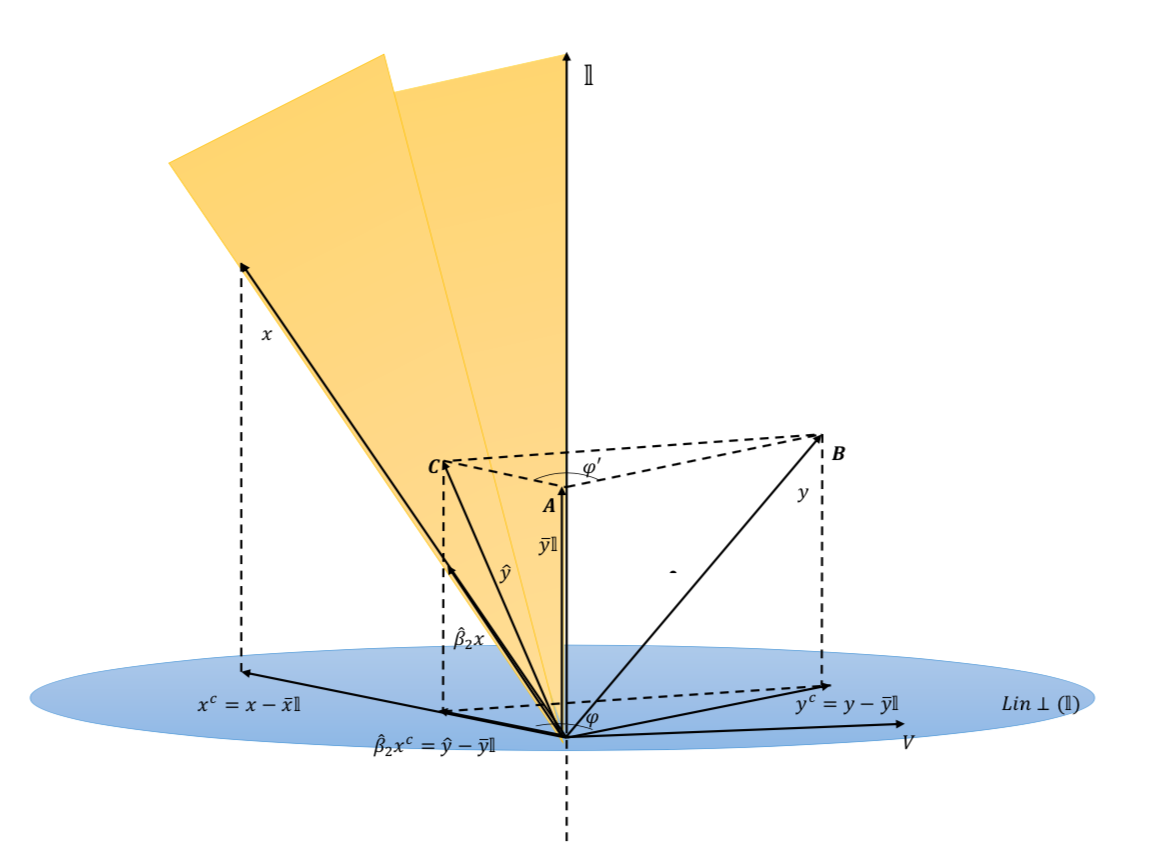
\includegraphics[width=0.24\paperwidth]{ols.png}

$ \sCorr{(x;y)} = \frac{\sum\limits_{i=1}^n(x_i - \bar{x})(y_i - \bar{y})}{\sqrt{\sum\limits_{i=1}^n (x_i - \bar{x})^2 \sum\limits_{i=1}^n(y_i - \bar{y})^2}}$ \\
\\
Проекция $y$ на $Lin(\mathbbm {1}; x)$: $\hat{y} = \hat{\beta}_1\mathbbm {1} + \hat{\beta}_2x^c$ \\
\\
Проекция $x$ и $y$ на $Lin \bot (\mathbbm {1})$: $x^c = x - \bar{x}\mathbbm {1} = \sqrt{\sum\limits_{i=1}^n(x_i - \bar{x})^2}, y^c = y - \bar{y}\mathbbm {1} = \sqrt{\sum\limits_{i=1}^n(y_i - \bar{y})^2}$\\
Проекция $x$ и $y$ на $Lin \bot (\mathbbm {1})$: $x^c = x - \bar{x}\mathbbm {1} = \sqrt{\sum\limits_{i=1}^n(x_i - \bar{x})^2}$\\
\\
Проекция $y^c$  на $Lin(x^c)$: $ {\beta}_2x^c = \hat{y} - \bar{y}\mathbbm {1}$\\
\\
Проекция $x^c$  на $Lin(\mathbbm {1})$: 0\\
\\
Проекция $x^c$  на $Lin \bot (\mathbbm {1})$: $x^c$\\
%\item $\bar{V} \bot \mathbbm {1}:V_1*1+V_2*1+V_3*1 = 0 \Rightarrow \sum V = 0 \Rightarrow V = 0 $



\begin{center}
\begin{math}
\begin{tabular}{r  l}
\hline
TSS = & $\sum\limits_{i=1}^n (y_i-\bar{y})^2 = ESS + RSS = |y- \bar{y}\mathbbm {1}|^2 = AB^2 = y^{c^2}$ \\
ESS = & $\sum\limits_{i=1}^n (\hat{y_i}- \bar{\hat{y}})^2 = AC^2$ \\
RSS = & $\sum\limits_{i=1}^{n}(y_i-\hat{y_i})^2 = \sum\limits_{i=1}^{n}e^2_i = BC^2$\\
$R^2$ = & $\frac{ESS}{TSS} = \frac{ \sVar{(\hat{y})}}{ \sVar{(y)}} = \frac{AC^2}{AB^2} = \cos{(\varphi')} = \sCorr^2{(y;\hat{y})} = \sCorr^2{(y;x)}$\\
\hline
\end{tabular}
\end{math}
\end{center}
%%\textbf{Сумма квадратов отклонений регрессии \textit{(ESS)}}
%%$$ESS = \sum\limits_{i=1}^n (\hat{Y}- \bar{Y})^2$$\\
%%\textbf{Полная сумма квадратов отклонений от среднего \textit{(TSS)}}
%%$$TSS = \sum\limits_{i=1}^n (Y-\bar{Y})^2 = ESS + TSS$$\\
%%\textbf{Коэффициент детерминации регрессии \textit{(R^2)}}
%%$$R^2 = \frac{ESS}{TSS} = 1 - \frac{RSS}{TSS}$$

\subsection*{\textbf{1.2 Теорема Гаусса - Маркова для случая парной регрессии}}
\underline{\textsc{\textit{Зачем она нужна?}}} \textit{Для получения дополнительной информации о характеристиках распределения оценок $\hat{\beta}_1, \hat{\beta}_2$} \\
\begin{tcolorbox}[colback=red!5!white,colframe=red!75!black]
\textbf{\underline{Теорема 1.2} Гаусса - Маркова для случая парной регрессии }. Если для модели $\hat{y}_i=\hat{\beta}_1 + \hat{\beta}_2x_i + \varepsilon_i, i = 1,...,n$ выполняются следующие условия:

1) Строится регрессия $y$ на $x$

2) Не все $x_i$ равны между собой

3) %$\forall \varepsilon_i, \E{(\varepsilon_i)}=0, \qquad i = 1, ..., n$
Математическое ожидание от любой ошибки регрессии равно 0

4) %$\forall \varepsilon_i \: \Var{(\varepsilon_i)}=\sigma_{\varepsilon_i}^2 \qquad \forall i$
Дисперсия от любой ошибки регрессии равна $\sigma_{\varepsilon}^2$


5) $\Cov(\varepsilon_i, \varepsilon_j) = 0$ - отсутствие автокорреляции, \\
то МНК - оценки $\hat{\beta}_1$ и  $\hat{\beta}_2$ являются \textit{BLUE}
 \end{tcolorbox}

\begin{center}
\begin{tabular}{l  l}
\hline
\textbf{B}est (наилучшие) &  для любых $\hat{\beta_i}$ верно: \\
 & $MSE(\hat{\beta_i})\le MSE(\tilde{\beta_i}))$\\
\textbf{L}inear (линейные) & Оценки линейные по $y$\\
\textbf{U}nbiased (несмещенные) \textbf{E}stimator (оценки) & $ \E{(\hat{\beta_i})}=\beta_i$\\
\hline
\end{tabular}
\end{center}

\begin{tcolorbox}[colback=blue!5!white,colframe=blue!75!black]
\textbf{\underline{Утверждение 1.2}} Если условия теоремы Гаусса - Маркова выполнены, то дисперсии МНК оценок:
\begin{center}
\begin{tabular}{r  l}
$\Var{(\hat{\beta}_1)} = \sigma_{\varepsilon}^2 \frac{\sum\limits_{i=1}^n {x_i}^2}{n\sum\limits_{i=1}^n ({x_i}- \bar{x})^2} \qquad \Var{(\hat{\beta}_2}) = \frac{ \sigma_{\varepsilon}^2}{\sum\limits_{i=1}^n ({x_i}- \bar{x})^2}$
\end{tabular}
\end{center}
а их ковариация:
\begin{center}
\begin{tabular}{r  l}
$\Cov(\hat{\beta}_1,\hat{\beta}_2) = - \frac{\bar{x}\sigma_{\varepsilon}^2}{n\sum\limits_{i=1}^n(x_i- \bar{x})^2}$
\end{tabular}
\end{center}
 \end{tcolorbox}


\subsection*{\textbf{1.3 Предположение о нормальном распределении случайной ошибки в рамках классической линейной регрессии}}

\begin{tcolorbox}[colback=green!5!white,colframe=green!75!black]
\textbf{\underline{Утверждение 1.3.1}} Если верно, что $\varepsilon_i \sim N(0, \sigma_{\varepsilon}^2)$, $i = 1...n$, то МНК-оценки коэффициентов парной регрессии также имеют нормальное распределение, причём $\hat{\beta_1} \sim N(\beta_1, Var(\hat{\beta_1}))$, $\hat{\beta_2} \sim N(\beta_2, Var(\hat{\beta_2}))$.
\end{tcolorbox}
\begin{tcolorbox}[colback=green!5!white,colframe=green!75!black]
\textbf{\underline{Утверждение 1.3.2}} $ \hat{\sigma}^2_{\varepsilon} = \frac{RSS}{n-2}$ является несмещённой оценкой для $\sigma^2_\varepsilon$.
\end{tcolorbox}
\begin{tcolorbox}[colback=green!5!white,colframe=green!75!black]
\textbf{\underline{Утверждение 1.3.3}} $\frac{RSS}{\sigma^2_\varepsilon} \sim \chi^2_{n-2} $ для парной регрессии.
\end{tcolorbox}
\begin{tcolorbox}[colback=green!5!white,colframe=green!75!black]
\textbf{\underline{Утверждение 1.3.4}} Оценки $\hat{\beta_1}$ и $\hat{\sigma}^2_{\varepsilon}$, $\hat{\beta_2}$ и $\hat{\sigma}^2_{\varepsilon}$ являются независимыми.
\end{tcolorbox}

\subsubsection*{\textbf{1.3.1 Проверка гипотезы о конкретном значении коэффициентов парной регрессии}}
\[H_0: \beta_2 = \beta_2^0\]
\[H_a: \beta_2 \neq \beta_2^0\]
Если $|t = \frac{\hat{\beta}_2 - \beta_2^0}{\sqrt{\hat\Var({\hat{\beta}_2})}}| > t^{cr}$ (при уровне значимости $\alpha/2$ и $n-2$ степенях свободы), то гипотеза $H_0$ отвергается в пользу гипотезы $H_a$.\\
Если значение $|t = \frac{\hat{\beta}_2 - \beta_2^0}{\sqrt{\hat\Var({\hat{\beta}_2})}}| < t^{cr}$ (при уровне значимости $\alpha/2$ и $n-2$ степенях свободы), то гипотеза $H_0$ не отвергается.\\

\subsubsection*{\textbf{1.3.2 Проверка гипотезы о значимости коэффициентов парной регрессии}}
\[H_0: \beta_2 = 0\]
\[H_a: \beta_2 \neq 0\]
Если значение $|t = \frac{\hat{\beta}_2}{\sqrt{\hat\Var{(\hat{\beta}_2)}}}| > t^{cr}$ (при уровне значимости $\alpha/2$ и $n-2$ степенях свободы), то гипотеза $H_0$ отвергается, значит, $\beta_2$ значим.\\
\\%% \textit{\underline{Интерпретация оценки}: при увеличении $X$ на одну единицу $Y$ увеличивается на $\hat{\beta}_2$ единиц при прочих равных условиях}\\
Если значение $|t = \frac{\hat{\beta}_i}{\sqrt{\hat\Var{(\hat{\beta}_2)}}}| < t^{cr}$ (при уровне значимости $\alpha/2$ и $n-2$ степенях свободы), то гипотеза $H_0$ не отвергается, значит, $\beta_2$ не значим.\\
\\
\textbf{Доверительный интервал}\\
\[[\hat{\beta}_2 - t^{cr}\sqrt{\hat\Var{(\hat{\beta}_2)}};\hat{\beta}_2 + t^{cr}\sqrt{\hat\Var{(\hat{\beta}_2)}}]\]
Если доверительный интервал включает в себя нуль, то этот коэффициент не значим, при уровне значимости $\alpha$. \\
В обоих случаях $t^{cr}$ рассчитывается на уровне значимости $\alpha/2$ с $n-2$ степенями свободы.
\subsubsection*{\textbf{1.3.3 Прогнозирование по модели парной регрессии и его точность}}
\begin{itemize}
\item \textbf{Доверительный интервал для среднего прогноза}\\
$\hat\Var(\hat{y}_{n+1})=\hat\Var(\hat{\beta_1}+\hat{\beta_2}x_{n+1})= \hat{\sigma}^2_\varepsilon[\frac{1}{n}+\frac{(x_{n+1}-\bar{x})^2}{\sum\limits_{i = 1}^n(x_i - \bar{x})^2}]$ \\
\doublespacing
$P(\hat{\beta_1}+\hat{\beta_2}x_{n+1} - t_{\alpha/2, n-2}\sqrt{\hat\Var(\hat{y}_{n+1})} \le E(y_{n+1}|x=x_{n+1}) \le \hat{\beta_1} +$ \\
$\hat{\beta_2}x_{n+1} + t_{\alpha/2, n-2}\sqrt{\hat\Var(\hat{y}_{n+1})}) = 1-\alpha$ \\

\onehalfspacing
\item \textbf{Доверительный интервал для индивидуального прогноза}\\
$\hat\Var(y_{n+1}) = \hat\Var(\hat{\beta_1}+\hat{\beta_2}x_{n+1} + \varepsilon_{n+1}) = \hat{\sigma}^2_\varepsilon[1+\frac{1}{n}+\frac{(x_{n+1}-\bar{x})^2}{\sum\limits_{i = 1}^n(x_i - \bar{x})^2}]$ \\
$P(\hat{\beta_1}+\hat{\beta_2}x_{n+1} - t_{\alpha/2, n-2}\sqrt{\hat\Var(y_{n+1})} \le y_{n+1} \le \hat{\beta_1}+\hat{\beta_2}x_{n+1} + $ \\
\doublespacing
$t_{\alpha/2, n-2}\sqrt{\hat\Var(y_{n+1})}) = 1-\alpha$ \\

\onehalfspacing
\item \textbf{Доверительный интервал дисперсии ошибок регрессии}\\

$P(\frac{RSS}{\chi^2_{\alpha/2, n-2}} \le \sigma^2_\varepsilon \le \frac{RSS}{\chi^2_{1-\alpha/2, n-2}}) = 1-\alpha$
\end{itemize}

\subsubsection*{\textbf{1.3.4 Проверка гипотезы о нормальности распределения}}
\begin{itemize}
\item \textbf{Критерий Колмогорова - Смирнова}\\
\\
\underline{\textsc{\textit{Когда используется?}}} \textit{Выборка состоит из достаточно большого количества наблюдений $n$} \\
\[H_0: F(t) = G(t) \text{ для любого t} \]
\[H_a: F(t) \neq G(t) \text{ при некотором t} \]
С использованием таблиц:
\[ J = \frac{mn}{d}\max\limits_{-\infty<t<\infty}|F_m(t) - G_n(t)| \]
где $F_m(t)$ и $G_m(t)$ -- эмпирические функции распределения для выборок $x_1,...,x_m$ и $y_1,...,y_n$, а именно:\\
\begin{center}
\begin{math}
\begin{tabular}{r  l}
$F_m(t) =$ & $\frac{\text{Число элементов в первой выборке, не превышающих \textit{t}}}{m}$\\
$G_n(t) =$ & $\frac{\text{Число элементов во второй выборке, не превышающих \textit{t}}}{n}$ \\
\end{tabular}
\end{math}
\end{center}

$d$ — $\text{НОД}(m,n)$, $m$ и $n$ — общее количество элементов в первой и второй выборке соответственно.\\

Статистика имеет специальное распределение $D$ при верной $H_0$:
\begin{center}
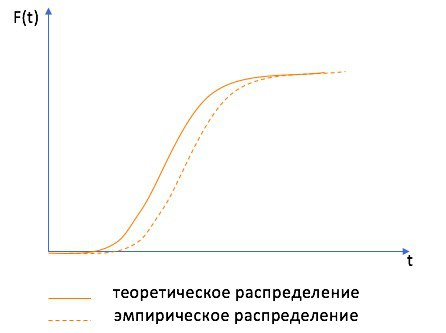
\includegraphics[width=0.15\paperwidth]{kstest.jpg}
\end{center}
%$H_0$ отвергается в пользу $H_a$ при условии, что $J \geq j_{\alpha}$ (в противном случае не отвергается).\\
% \\
%Без использования таблиц, $s > 0$(и 0 в противном случае):
%\[P(\sqrt{m}J_0 < s) = 1 - 2\sum\limits_{k = 0}^{\infty}(-1)^{k}e^{-2k^2s^2}\]
%При $min(m,n) \to \infty$ гипотеза $H_0$ отвергается в пользу $H_a$ при условии, что $J \geq q_{\alpha}^*$, где $q_{\alpha}^*$ определяется из соотношения $Q(q_{\alpha}^*) = \alpha$, а $Q(s) = 1 - \sum\limits_{k = - \infty}^{-\infty}(-1)^ke^{-2k^2s^2}$ для $s>0$ (и 0 противном случае).
%\\
\item\textbf{Тест Харке - Бера}
%\\
\underline{\textsc{\textit{Когда используется?}}} \textit{Выборка состоит из достаточно большого количества наблюдений $n$}
\[H_0: s = 0, k = 3\]
\[H_a: s \neq 0, k \neq 3\]
\\
Тестовая статистика:
\[JB = \frac{n}{6}(s^2+\frac{1}{4}(k - 3)^2) \sim \chi^2_2\]
Коэффициент асимметрии: $s = \frac{1}{n}\sum\limits_{i = 1}^n\frac{(x_i - \bar{x})^3}{\hat{\sigma}^3}$, $\hat{\sigma}^2=\frac{1}{n}\sum\limits_{i = 1}^n{(x_i - \bar{x})}$\\
\\
\textit{Для симметричных распределений, в том числе нормального, этот показатель равен нулю.}\\
\\Коэффициент эксцесса: $k = \frac{1}{n}\sum\limits_{i = 1}^n{\frac{(x_i - \bar{x})^4}{\hat{\sigma}^4}}$\\
\textit{Для нормального распределения этот показатель равен 3.}\\
\\
Если $JB > \chi^2_2$ при выбранном уровне значимости, то гипотеза отвергается.\\

\item \textbf{Тест Шапиро - Уилка}\\
\\
\underline{\textsc{\textit{Когда используется?}}} \textit{Выборка состоит из небольшого количества наблюдений $n$}
\[H_0: x_1,...,x_n \text{-- выборка из нормального распределения}\]
\[H_a: x_1,...,x_n \text{-- выборка не из нормального распределения}\]
\\
Тестовая статистика:
\[W=\frac{(\sum\limits_{i = 1}^n{{\alpha}_{(i)}x_{i}})^2}{\sum\limits_{i = 1}^n{(x_{(i)} - \bar{x})^2}} \sim W_\alpha\]
Вектор коэффициентов: ${\alpha}_{(i)} = \frac{m^TV^{-1}}{m^TV^{-1}V^{-1}m}$\\

$m$ -- вектор математических ожиданий порядковых статистик нормального распределения; \\
$V$ -- ковариационная матрица этих порядковых статистик размера n*n.\\
\\
Для небольших $n$ коэффициенты $\alpha_{(i)}$ берутся из таблиц.\\
\\
Если $W<W_\alpha$, то гипотеза $H_0$ отвергается.
\end{itemize}

\columnbreak

\section*{2.0 Линейная регрессия с несколькими объясняющими переменными (множественная регрессия)}
\begin{tcolorbox}[colback=red!5!white,colframe=red!75!black]
Модель \textbf{множественной линейной регрессии} имеет следующий вид:
 $$y_i={\beta}_1 +{\beta}_2x_{i2} + ... + \beta_kx_{ik} + {\varepsilon}_i, \quad i = 1,...,n$$
 где $i$ -- номер наблюдения, а ${\varepsilon}_i$ -- ошибки регрессии
\end{tcolorbox}

\subsection*{\textbf{2.1 Формула для  МНК - оценок коэффициентов множественной линейной регрессии}}
\underline{\textsc{\textit{Зачем она нужна?}}} \textit{Для нахождения оценки коэффициентов $\hat{\beta}_i$}\\
%$RSS \to \min\limits_{\hat{\beta}}$, где $RSS = \sum\limits_{i=1}^{n}e_i^2$
%%$\Longrightarrow\\
\[\hat{\beta} = (X^TX)^{-1}X^Ty\] \\

\[\hat{\beta}_m = \frac{\det{\begin{pmatrix}
\sCov{\begin{pmatrix}
  \ x_{1i}& \ & \ x_{1i}&\\
  \ x_{2i}& \ & \ x_{2i}&\\
  \ ...& \ ;& \ ...&\\
  \ x_{mi}& \ &\ y_i&\\
  \ x_{ki}&\ & \ x_{ki}\
  \end{pmatrix}}\end{pmatrix}}}{\det{\begin{pmatrix}
\ \sVar{\begin{pmatrix}
  \ x_{1i}& \\
  \ x_{2i}& \\
  \ ...& \\
  \ x_{mi}& \\
  \ x_{ki}&
  \end{pmatrix}}\end{pmatrix}}}\]
\\
\textsc{\textit{Показатель качества подгонки множественной регрессии:}} \\
\\
\begin{tabular}{r  l}\
$ 1) R^2 = \frac{ESS}{TSS} = \hat{r}^2_{y,\hat{y}}, R^2 \in [0;1]; \qquad 2) R^2_{adj} = 1 - \frac{RSS(n-1)}{TSS(n-k)}$
\end{tabular}
\\
$R^2_{adj}$ -- показатель качества, штрафующий за включение слишком большого количества переменных в модель.

\subsection*{\textbf{2.2 Теорема Гаусса - Маркова для случая множественной регрессии}}
\begin{tcolorbox}[colback=red!5!white,colframe=red!75!black]
\textbf{\underline{Теорема 2.2} Гаусса - Маркова для случая множественной регрессии}\\
Если для модели $y_i={\beta}_1 +{\beta}_2x_{i2} + ... + \beta_kx_{ik} + {\varepsilon}_i, i = 1,...,n$ выполнены условия: \\
1) Модель правильно специфицирована, то есть в нее включен только необходимый $x$, объясняющий $y$

2) Нет линейной зависимости между факторами

3) %$\forall \varepsilon_i, \E{(\varepsilon_i)}=0, \qquad i = 1, ..., n$
Математическое ожидание от любой ошибки регрессии равно 0

4) %$\forall \varepsilon_i \: \Var{(\varepsilon_i)}=\sigma_{\varepsilon_i}^2 \qquad \forall i$
Дисперсия от любой ошибки регрессии равна $\sigma_{\varepsilon}^2$

%5) $\forall \varepsilon_i \:\varepsilon_i \sim N(0, \sigma^2_{\varepsilon_i})$ -- случайный член гомоскедастичен

5) $ \Cov{(\varepsilon_i, \varepsilon_j)} = 0$ -- отсутствие автокорреляции, \\
то оценки МНК $\hat{\beta} = (X^TX)^{-1}X^Ty$ являются BLUE.
\end{tcolorbox}

\begin{tcolorbox}[colback=blue!5!white,colframe=blue!75!black]
Если выполнены условия ТГМ, то дисперсии МНК оценок следующие: \\
$$\Var{(\hat{\beta_j})}= \sigma^2_{\varepsilon}(X^TX)^{-1}_{jj} \quad j = 0,..,k$$
\end{tcolorbox}

\subsection*{\textbf{2.3 Предположение о нормальном распределении случайной ошибки в рамках классической линейной регрессии}}
\begin{tcolorbox}[colback=green!5!white,colframe=green!75!black]
\textbf{\underline{Теорема 2.3} Фишера}\\
Если выполнены условия Теоремы Гаусса - Маркова и $\varepsilon \sim N(0, \sigma^2_{\varepsilon}I)$, то \\
1) Оценки МНК $\hat{\beta} \sim N(\beta, \sigma^2_{\varepsilon}(X^TX)^{-1})$ \\
2) $\frac{RSS}{\sigma^2_{\varepsilon}} \sim \chi^2_{n-k}$ \\
3) $\hat{\beta}$ и $RSS$ независимы
\end{tcolorbox}

\begin{tcolorbox}[colback=green!5!white,colframe=green!75!black]
\textbf{\underline{Утверждение 2.3.1}} $\hat{\sigma}^2_{\varepsilon} = \frac{RSS}{n-k}$ является несмещённой оценкой для $\sigma^2_{\varepsilon}.$
\end{tcolorbox}

\columnbreak

\subsection*{\textbf{2.4 Проверка гипотез в случае множественной регрессии для модели $y_i={\beta}_1 +{\beta}_2x_{i2} + ... + \beta_kx_{ik} + {\varepsilon}_i$}}
\subsubsection*{\textbf{2.4.1 Проверка гипотезы о конкретном значении коэффициентов множественной регрессии}}
\[H_0: \beta_j = \beta_j^0\]
\[H_a: \beta_j \ne \beta_j^0\]
\\
Тестовая статистика рассчитывается как:
\[t = \frac{\hat{\beta_j} - \beta_j^0}{\sqrt{\hat{\sigma}^2_{\varepsilon}(X^TX)^{-1}_{jj}}} \sim t_{n-k}\]
Если $|t| > t^{cr}$(при уровне значимости $\alpha/2$ и $n-k$ степеней свободы), то гипотеза $H_0$ отвергается.  \\
\\
Для проверки \textit{гипотезы о значимости} используют $\beta_j^0 = 0$. \\
\\
\textbf{Доверительный интервал для проверки гипотезы:} \\
\[[\hat{\beta_j} - t^{cr}\sqrt{\hat{\sigma}^2_{\varepsilon}(X^TX)^{-1}_{jj}}; \hat{\beta_j} + t^{cr}\sqrt{\hat{\sigma}^2_{\varepsilon}(X^TX)^{-1}_{jj}}]\]
$t^{cr}$ рассчитывается на уровне доверия $\alpha/2$ с $n-k$ степенями свободы.\\
Если в интервал входит нуль, то основная гипотеза не отвергается.
\subsubsection*{\textbf{2.4.2 Проверка общей линейной гипотезы о коэффициентах множественной регрессии}}
\[H_0: Q\beta=q\]
\[H_a: Q\beta \ne q\]
Инкорпорируем ограничение в регрессию и рассчитываем $R^2_r$ и $RSS_r$ \\
Также оцениваем регрессию без ограничений и получаем $R^2_{ur}$ и $RSS_{ur}$
\\
Тестовая статистика рассчитывается как:
\[F = \frac{(RSS_r - RSS_{ur})/q}{RSS_{ur}/(n-k)} = \frac{(R^2_{ur}-R^2_{r})/q}{(1-R^2_{ur})/(n-k)} \sim F_{q, n-k}\] \\
Если при выбранном уровне значимости $\alpha$ верно, что $F > F^{cr}$, то основная гипотеза $H_0$ отвергается.

\subsubsection*{\textbf{2.4.3 Проверка гипотезы об адекватности регрессии}}
\[H_0: \beta_2 = ... = \beta_k = 0\]
\[H_a: \text{хотя бы один коэффициент } \beta_j \text{ отличен от нуля}, j=2,..,k\]
\\
Тестовая статистика рассчитывается как:
\[F = \frac{ESS/(k-1)}{RSS/(n-k)} = \frac{R^2/(k-1)}{(1-R^2)/(n-k)} \sim F_{k-1, n-k}\] \\
Если при выбранном уровне значимости $\alpha$ верно, что $F > F^{cr}$, то основная гипотеза $H_0$ отвергается, регрессия адекватна.

%%\subsection*{\textbf{2.5 Метод максимального правдоподобия (LR)}}
%%\underline{\textsc{\textit{Зачем он нужен?}}} \textit{Для реальных данных, на которых не выполняется условие Гаусса - Маркова}\\
%%$$L(x_1,..., x_n | {\theta})=P(X_1 =x_1,...,X_n = x_n | {\theta}) \to \max\limits_{\theta}$$
%%${\theta}$ - вектор оцениваемых параметров\\
%%На практике используется логарифмитеческая функция правдоподобия:
%%$$l(x_1,..., x_n | {\theta}) = \ln L(x_1,...,x_n |  {\theta}) \to \max\limits_{\theta}$$
%%\begin{tcolorbox}[colback=red!5%%!white,colframe=red!75!black]
%%\textbf{Алгоритм нахождение ММП - оценки параметра $\lambda$\\}
%1. $L(x_1,..., x_n | {\lambda})=P(X_1 =x_1,...,X_n = x_n | {\lambda}) = P(X_1 = x_1, ...,X_n=x_n | {\lambda}) =P(X_1 = x_1 | {\lambda})*...*P(X_n = x_n | \lambda)$\\%
%2. $l(x_1,..., x_n | {\lambda}) = \ln{L(x_1,...,x_n |  {\lambda})}$\\
%3. $l'_{\lambda}(x_1,..., x_n | {\lambda}) = 0$\\
%4. Выражаем ${\lambda}$\\
%5.  $l''_{\lambda}(x_1,..., x_n | {\lambda})$, если $l''_{\lambda} < 0$, то условие максимума выполнено и $\hat{\lambda}_{LR}$ \\
%%\end{tcolorbox}

%\subsubsection*{2.5.1 Проверка линенйных гипотез с помощью теста отношения правдоподобия}
%\underline{\textsc{\textit{Когда используется?}}} \textit{Для проверки гипотез линейных и нелинейных ограничений на коэффициенты регрессии}
%$$LR = -2\ln{\lambda} = 2(l(\hat{\beta},\hat{\sigma}^2)-l((\tilde{\beta},\tilde{\sigma}^2))$$
%$\hat{\beta},\hat{\sigma}^2$ - модель без ограничений\\
%$\tilde{\beta},\tilde{\sigma}^2$ - модель с ограничениями\\

\subsection*{\textbf{2.5 Фиктивные (dummy) переменные}}
\begin{tcolorbox}[colback=red!5!white,colframe=red!75!black]
\textbf{Фиктивные (dummy) переменные} -- переменные которые принимают только два значения, обычно 0 и 1.
\end{tcolorbox}
\subsubsection*{2.5.1 Проверка гипотез о структурной устойчивости регрессии (о единой зависимости)}
\begin{itemize}
\item \textbf{Тест Чоу} \\
\\
%$\left[
      %\begin{gathered}
       % D_i = 1, i = 1,..,n_1, то y_i=({\beta}_1+\delta_1) +({\beta}_2+\delta_2)x_{i2} + ... + {\varepsilon}_i\\
        %D_i = 0, i = n_1+1,..,n, то y_i={\beta}_1 +{\beta}_2x_{i2} + ... + \beta_kx_{ik} + {\varepsilon}_i\\
      %\end{gathered}
%\right.$ \\
При $D_i = 1, i = 1,..,n_1$ уравнение регрессии имеет вид:
\[y_i=({\beta}_1+\delta_1) +({\beta}_2+\delta_2)x_{i2} + ... + {\varepsilon}_i\]
При $D_i = 0, i = n_1+1,..,n$ уравнение регрессии имеет вид:
\[y_i={\beta}_1 +{\beta}_2x_{i2} + ... + \beta_kx_{ik} + {\varepsilon}_i \]
\columnbreak

Пусть $\beta'_j = \beta_j+\delta_j, j = 0,..,k$. Тогда гипотеза будет следующая:
\[H_0: \beta_i = \beta'_i, i = 0,..,k\]
\[H_a: \text{существует такое j, что } \beta_j \ne \beta_j'\]
\\
Тестовая статистика рассчитывается как:
\[F = \frac{(RSS_{pooled} - RSS_1-RSS_2)/k}{(RSS_1+RSS_2)/(n-2k)} \sim F_{k, n-2k}\]
где $RSS_{pooled}$ -- $RSS$ в регрессии, оцененной по всем n наблюдениям; \\
$RSS_1$ -- $RSS$ в регрессии, оцененной по наблюдениям $i=1,...,n_1$; \\
$RSS_2$ -- $RSS$ в регрессии, оцененной по наблюдениям $i=n_1+1,...,n_1+n_2$.\\

\item \textbf{С помощью dummy переменных}
\\
\end{itemize}
\[H_0: \delta_1 = ... = \delta_k = 0 \text{ -- зависимость едина}\]
\[H_a: \delta^2_1 + ... + \delta^2_k \ne 0 \text{ -- зависимость не едина}\]
\\
Регрессия без ограничений: $y_i={\beta}_1 + \delta_1D_i +{\beta}_2x_{i2} + \delta_2D_ix_{i2} + ... + {\varepsilon}_i$ \\
Регрессия с ограничениями: $y_i={\beta}_1 +{\beta}_2x_{i2} + ... + \beta_kx_{ik} + {\varepsilon}_i$ \\
\\
Тестовая статистика рассчитывается как:
\[F = \frac{(RSS_r - RSS_{ur})/k}{RSS_{ur}/(n-2k)} \sim F_{k, n-2k}\]
\\
В обоих случаях, если при выбранном уровне значимости $\alpha$ верно, что $F > F^{cr}$, то основная гипотеза $H_0$ отвергается, и зависимость не едина.


\section*{3.0 Выбор функциональной формы модели}
\subsubsection*{3.0.1 Формы модели}
\begin{itemize}
\item \textbf{Линейная модель}
\[y_i = \beta_1 + \beta_2x_{i2}+...+\beta_{k}x_{ik}+\varepsilon_i\]
\begin{center}
    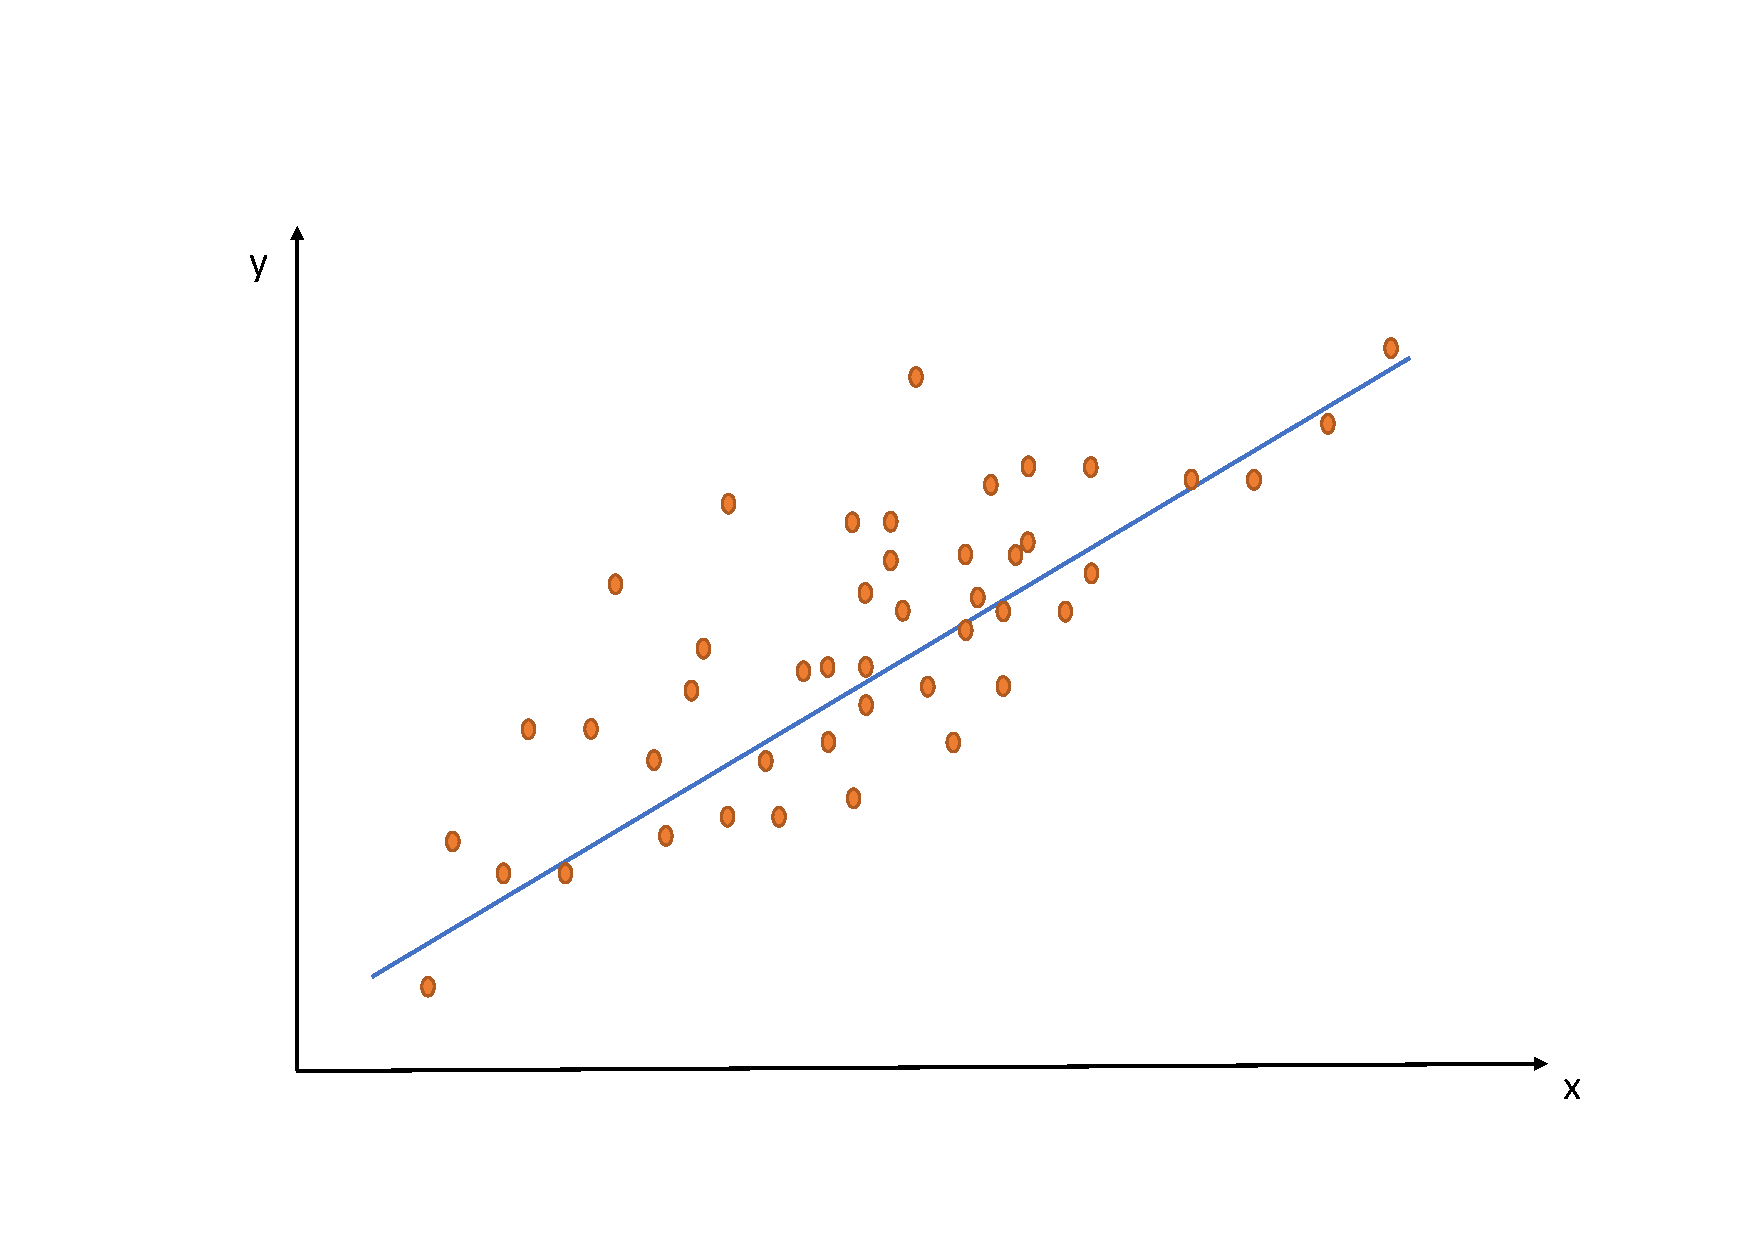
\includegraphics[width=0.2\paperwidth]{linear.pdf}
\end{center}

\textit{Интерпретация оценки коэффициентов линейной регрессии}:\\
Если коэффициент $\beta_j$ значим, то при изменении $x_j$ на одну единицу $y$ изменится на $\hat{\beta}_j$ единиц (в сторону увеличения при положительной оценке и в сторону уменьшения при отрицательной). \\
\item \textbf{Полулогарифмическая модель (модель с постоянным темпом роста)}
\[\ln{y_i} = \beta_1 + \beta_2x_{i2}+...+\beta_kx_{ik}+\varepsilon_i\]
\textit{Интерпретация оценки коэффициентов полулогарифмической регрессии}:
Если коэффициент $\beta_j$ значим, то при изменении $x_j$ на одну единицу $y$ изменится на $\hat{\beta}_j\cdot 100\%$ \\
\item \textbf{Линейная в логарифмах модель (модель с постоянной эластичностью)}
\[\ln{y_i} = \beta_1 + \beta_2\ln{x_{i2}}+...+\beta_k\ln{x_{ik}}+\varepsilon_i\]
\textit{Интерпретация оценки коэффициентов логарифмической регрессии}:\\
Если $\beta_j$ значим, то при изменении $x_j$ на 1\%  $y$ изменится на $\hat{\beta}_j\%$
\end{itemize}
\subsubsection*{3.0.2 Выбор между моделями}
\begin{itemize}
\item \textbf{Тест Бера и МакАлера}\\
\\
\underline{\textsc{\textit{Когда используется?}}} \textit{Для выбора между полулогарифмической и линейной моделями}\\
\textit{Шаг 1}. Нахождение оцененных значений зависимой переменной в каждой из этих моделей ($\hat{\ln{y}}$ и $\hat{y}$).\\
\textit{Шаг 2}. Оценка вспомогательных регрессий
\[\exp{(\hat{\ln{y_i})}=\beta_1 + \beta_2x_{i2}+...+\beta_kx_{ik}+\upsilon_{1}}\]
\[\ln{\hat{y_i}}=\beta_1 + \beta_2x_{2i}+...+\beta_kx_{ik}+\upsilon_{2}\]
и сохранение остатков регрессий $\hat{\upsilon_1}$ и $\hat{\upsilon_2}$\\
\textit{Шаг 3}. Оценка моделей
\[\ln{y_i} = {\beta}_1 + \beta_2x_{2i}+...+\beta_kx_{ik} + {\theta}_1\hat{\upsilon_1} + \varepsilon_{i}\]
\[y_i ={\beta}_1 + \beta_2x_{i2}+...+\beta_kx_{ik} + {\theta}_2\hat{\upsilon_2} + \varepsilon_{i}\] и проверка следующих гипотез о значимости c помощью $t$-тестов:
\begin{center}
\begin{tabular}{r  l}
$H_0: \theta_1 = 0 \qquad \qquad \qquad$ &$H_0: \theta_2 = 0$ \\
$H_a: \theta_1 \ne 0 \qquad \qquad \qquad$&$H_a: \theta_2 \ne 0$
\end{tabular}
\end{center}

Если коэффициент $\theta_1$ не значим, то выбирается полулогарифмическая модель. Если коэффициент $\theta_2$ не значим, то выбирается линейная модель. Если оба коэффициента $\theta_1$ и $\theta_2$ одновременно значимы или не значимы, модель выбрать нельзя.  \\
\item \textbf{МакКиннона, Уайта и Дэвидсона}\\
\\
\underline{\textsc{\textit{Когда используется?}}} \textit{Для выбора между полулогарифмической и линейной моделями}\\
\textit{Шаг 1}. Нахождение оцененных значений зависимой переменной в каждой из этих моделей ($\hat{\ln{y}}$ и $\hat{y}$).\\
\textit{Шаг 2}. Оценка вспомогательных регрессий
\[\ln{y_i} = {\beta}_1 + \beta_2x_{i2}+...+\beta_kx_{ik} + {\gamma}_1(\hat{y_i}-\exp{(\hat{\ln{y_i}})}) + \varepsilon_{i}\]
\[y_i ={\beta}_1 + \beta_2x_{i2}+...+\beta_kx_{ik} + {\gamma}_2(\ln{\hat{y_i}-\hat{\ln{y_i}}}) + \varepsilon_{i}\]
и проверка следующих гипотез о значимости c помощью $t$-тестов:
\begin{center}
\begin{tabular}{r  l}
$H_0: \gamma_1 = 0 \qquad \qquad \qquad$ &$H_0: \gamma_2 = 0$ \\
$H_a: \gamma_1 \ne 0 \qquad \qquad \qquad$&$H_a: \gamma_2 \ne 0$
\end{tabular}
\end{center}

Если коэффициент $\gamma_1$ не значим, то выбирается полулогарифмическая модель. Если коэффициент $\gamma_2$ незначим, то выбирается линейная модель. Если оба коэффициента $\gamma_1$ и $\gamma_2$ одновременно значимы или не значимы, модель выбрать нельзя.  \\
\\
\textit{Также данный тест используется для выбора между линейной и линейной в логарифмах моделями.}\\
\\
\textit{Шаг 1}. Нахождение оценённых значений зависимых переменных:$$\hat{\ln{y_i}} = \hat{\beta}_1 + \hat{\beta_2}\ln{x_{i2}}+...+\hat{\beta_k}\ln{x_{ik}}$$
\textit{Шаг 2}. Оценка вспомогательных регрессий
\[\ln{y_i} = {\beta}_1 + \beta_2\ln{x_{i2}}+...+\beta_k\ln{x_{ik}} + {\delta}_1(\hat{y_i}-\exp{(\hat{\ln{y_i}})}) + \varepsilon_i\]
\[y_i ={\beta}_1 + \beta_2x_{i2}+...+\beta_kx_{ik} + {\delta}_2(\ln{\hat{y_i}-\hat{\ln{y_i}})} + \varepsilon_i\]
и проверка следующих гипотез о значимости c помощью $t$-тестов:
\begin{center}
\begin{tabular}{r  l}
$H_0: \delta_1 = 0 \qquad \qquad \qquad$ &$H_0: \delta_2 = 0$ \\
$H_a: \delta_1 \ne 0 \qquad \qquad \qquad$&$H_a: \delta_2 \ne 0$
\end{tabular}
\end{center}

Если коэффициент ${\delta}_1$ не значим, то выбирается линейная в логарифмах модель. Если коэффициент ${\delta}_2$ не значим, то выбирается линейная модель. Если оба коэффициента ${\delta}_1$ и ${\delta}_2$ одновременно значимы или не значимы, модель выбрать нельзя.  \\
\item \textbf{Тест Бокса - Кокса}\\
\\
\underline{\textsc{\textit{Когда используется?}}}\textit{Для выбора функциональной формы модели}\\
\[y_i^{(\lambda)} = \beta_1 + \beta_2x_{i2}^{(\theta)} + \beta_kx_{ik}^{(\theta)} + \varepsilon_i\]
\[y_i^{(\lambda)} =
 \left\{
\begin{aligned}
\frac{y_i^\lambda - 1}{\lambda}, \qquad \lambda \neq 0 \\
\ln{y_i}, \qquad \lambda = 0
\end{aligned}
\right.\]

\[x^{(\theta)}_j =  \left\{ \begin{aligned}
\frac{x_j^{(\theta)} - 1}{\theta}, \qquad \lambda \neq 0 \\
\ln{x_j}, \qquad \theta = 0 \end{aligned}
\right.\]
\textit{Шаг 1}. Оценить коэффициенты $\beta_1, \beta_2, ..., \beta_k$\\
\textit{Шаг 2}. Оценить параметры $\lambda$ и $\theta$ c помощью метода максимального правдоподобия.\\
Для параметров $\lambda$ и $\theta$ можно проверять гипотезы с помощью теста отношения правдоподобия. В случае, когда в модели:
\begin{enumerate}
\item $\lambda = \theta$ (зависимая и независимая переменные преобразуются одинаково), можно проверить гипотезу:
\[H_0:\lambda = \theta =1 \text{(линейная модель)}\]
\[H_a:\lambda = \theta \neq 1\]
а также гипотезу:
\[H_0: \lambda = \theta =0 \text{(линейная в логарифмах модель)}\]
\[H_a: \lambda = \theta \neq 0\]
\item $\lambda = 1$ (преобразуются только независимые переменные), можно проверить гипотезу:
\[H_0: \theta = 1 \text{(линейная модель)}\]
\[H_a: \theta \neq 1\]
\item $\theta = 1$
(преобразуется только зависимая переменная), можно проверить гипотезу:
\[H_0: \lambda = 0 \text{(полулогарифмическая модель)}\]
\[H_a: \lambda \neq 0\]
\end{enumerate}

\item \textbf{Метод Зарембки}\\
\\
\underline{\textsc{\textit{Когда используется?}}}\textit{Для выбора между полулогарифмической и линейной моделями}\\
%\textit{Шаг 1.}Оценить исходные регрессии и найти их RSS: \\ %
%$$ y = \beta_1 + \beta_2x_1 + ... + \beta_kx_k +\epsilon \Longrightarrow RSS_1$$%
%$$ \ln(y) = \beta_1 + \beta_2x_1 + ... + \beta_kx_k +\epsilon \Longrightarrow RSS_2$$ %
\textit{Шаг 1.} \[y_{mg} = (\prod\limits_{i=1}^ny_i)^{1/n}\]
\textit{Шаг 2.} \[y_i* = \frac{y_i}{y_{mg}}\]
\textit{Шаг 3.} Оценить новые регрессии: \\
\[y_i^* = \beta_1 + \beta_2x_{i2} + ... + \beta_{k}x_{ik} +\varepsilon_i\]
\[\ln(y_i^*) = \beta_1 + \beta_2x_{i2} + ... + \beta_{k}x_{ik} +\varepsilon_i\]
И получить $RSS_1$ и $RSS_2$ соответственно.\\
\textit{Шаг 4.} Проверить гипотезу:
$$H_0: \text{между двумя моделями нет статистической разницы}$$
$$H_a: \text{между моделями есть статистическая разница} $$
Статистика рассчитывается как:
\[\chi^2 = \frac{n}{2}|\ln\frac{RSS_1}{RSS_2}| \sim \chi^2_1\]
При $\chi^2 > \chi^2_{cr}$ гипотеза $H_0$ отвергается. Тогда из двух построенных моделей следует выбрать ту, для которой $RSS$ будет меньше.
\end{itemize}

\section*{4.0 Ошибки спецификации модели}
\subsection*{4.1 Невключение существенной переменной}
Предположим, что истинная модель -- $y = \beta_1 + \beta_2x + \beta_3z + \varepsilon$. \\
При этом, оценивается модель $y = \beta_1 + \beta_2x + \varepsilon$.\\
Тогда оценка МНК коэффициента $\beta_2$ будет смещенной во всех случаях, кроме: \\
$1) \beta_3 = 0;$\\
$2) \sCov(x, z) = 0$, т.е. когда пропущенный и включенный фактор не коррелируют. \\
Величина смещения равна $\beta_3\frac{\sCov(x, z)}{\sVar(x)}$\\ \\
\textbf{\textit{В матричном виде}}: \\
Если истинная модель -- $y = X\beta + Z\gamma + \varepsilon$, а оценивается модель $y = X\beta + \varepsilon$, то оценка МНК вектора $\beta$ будет смещенной во всех случаях, кроме: \\
$1) \gamma = 0;$\\
$2) X^TZ = O$, где $O$ -- нулевая матрица, т.е. невключенные факторы ортогональны включенным.\\
Величина смещения равна $(X^TX)^{-1}X^TZ\gamma$ \\
\\
Если же \textbf{в модель включены излишние переменные}, то уменьшается эффективность оценок (дисперсия оценок коэффициентов увеличивается, t-статистики уменьшаются), однако они будут несмещенными.

\subsection*{4.2 Тест Рамсея для выявления пропущенных переменных}
Исходная модель: $y_i = \beta_1 + \beta_2x_{i2} + ... + \beta_kx_{ik} +\varepsilon_i$ \\
\[H_0: \text{модель правильно специфицирована} \]
\[H_a: \text{модель неправильно специфицирована} \]
\textit{Шаг 1.} Оцениваем исходную модель, сохраняем $\hat{y}$ и $RSS_{r}$ \\
\textit{Шаг 2.} Оцениваем вспомогательную модель:
\[y_i = \beta_1 + \beta_2x_{i2} + ... + \beta_kx_{ik} + \alpha_2\hat{y_i}^2 + ... + \alpha_m\hat{y_i}^m +\varepsilon_i\]
и находим $RSS_{ur}$ \\
\textit{Шаг 3.} Проверяем гипотезу:
\[H_0: \alpha_2 = ... = \alpha_m = 0\]
\[H_a: \alpha_2^2 + ... + \alpha_m^2 > 0 \]
\\
Статистика рассчитывается как:
\[F = \frac{(RSS_r - RSS_{ur})/(m-1)}{RSS_{ur}/[n-k-(m-1)])} \sim F_{m-1, n-k-(m-1)}\]
\\
Если при выбранном уровне значимости $F>F^{cr}$, то $H_0$ отвергается, модель специфицирована неверно.

\section*{5.0 Мультиколлинеарность}
\begin{tcolorbox}[colback=purple!5!white,colframe=purple!75!black]
\textbf{Теоретическая мультиколлинеарность} -- линейная зависимость между столбцами матрицы $X$ (например, включение всего набора dummy переменных).\\
\textbf{Практическая мультиколлинеарность} -- "почти линейная зависимость"\ между столбцами матрицы $X$.
\end{tcolorbox}
\subsection*{5.1 Признаки и последствия мультиколлинеарности:}
1. Высокие стандартные ошибки и малые t-статистики коэффициентов влекут за собой незначимость коэффициентов; соответственно, невозможно разграничить влияние факторов. \\
2. Небольшие изменения в данных могут привести к большим изменениям в оценках коэффициентов.
\subsection*{5.2 Индикаторы наличия мультиколлинеарности:}
1. Анализ матрицы парных коэффициентов корреляции объясняющих факторов. Если по модулю элемент выше, чем 0.75, то это может свидетельствовать о м/к. \\
2. $VIF(x_j)= \frac{1}{1-R^2_j}$, где $R^2_j$ -- относится к регрессии фактора $x_j$ на все остальные факторы. Значение больше 6 может свидетельствовать о м/к. \\
3. $CN = \sqrt{\frac{\lambda_{max}}{\lambda_{min}}}$, где $\lambda$ -- собственные значения матрицы $x^Tx$. Значение больше 30 может свидетельствовать о м/к.
\subsection*{5.3 Методы борьбы с мультиколлинеарностью:}
1. Переход к другой функциональной форме модели (например, модель в логарифмах); \\
2. Метод пошагового исключения (с максимальным P-значением) или включения (с минимальным P-значением) по одной переменной, пока все коэффициенты не останутся значимыми; \\
3. Метод исключения нескольких переменных одновременно. При этом следует проверить гипотезу:
\[H_0: \beta_{i_1}=...=\beta_{i_r}=0\]
\[H_a: \beta^2_{i_1}+...+\beta^2_{i_r}\ne0\]
\columnbreak

4. PCA (метод главных компонент):
\begin{itemize}
\item {Каждый вектор $x_1,..,x_k$ центрируется: $\tilde{x}_{ij}=x_{ij}-\bar{x}_{j}$}
\item {Находятся собственные значения $\lambda_1>...>\lambda_k>0$ и собственные векторы $v_1,..,v_k$ матрицы $\tilde{X}^T\tilde{X}$}. Собственные векторы и являются главными компонентами.
\item {$v_1$ объясняет изменчивость исходных факторов на $\frac{\lambda_1}{\sum\limits_{i=1}^{k}\lambda_i}\times 100\%$, $v_2$ -- на $\frac{\lambda_1+\lambda_2}{\sum\limits_{i=1}^{k}\lambda_i}\times 100\%$ и т.д.}
\item {В конце оценивается регрессия $y$ на выбранные компоненты.}
\end{itemize}
5. Гребневая (Ридж) регрессия: использование вместо МНК-оценок Ridge-оценок, которые находятся путём минимизации $RSS + \lambda\sum\limits_{i=1}^{n}\beta_i^2 $ \\
6. LASSO регрессия: использование вместо МНК--оценок Lasso-оценок, которые находятся путём минимизации $RSS + \lambda\sum\limits_{i=1}^{n}|\beta_i| $ \\

\section*{6.0 Прогнозирование по регрессионной модели, оцененной по перекрестным данным}
\begin{itemize}
%%Индивидуальное предсказание вычисляется по формуле $\hat{\epsilon}_{n+1} = \epsilon_{n+1} - x_{n+1}^T(x^Tx)^{-1}x^T\epsilon$\\
%%$\hat{\beta} = \beta+{(x^Tx)}^{-1}x^T\epsilon$ \\
%% $\hat{Var}(\hat{\epsilon}_{n+1}) = %% %% {\hat{\sigma}^2}_{\epsilon}(1+{x^T}_{n+1}(x^Tx)^{-1}x_{n+1})$ \\ %%
\item{Доверительный интервал для индивидуального прогноза:}\\
\[[\hat{y}_{n+1} - t^{cr}\sqrt{\hat{\sigma}^2_\varepsilon(1+
x^T_{n+1}{(X^TX)}^{-1}x_{n+1})}; \hat{y}_{n+1} + \]
\[+ t^{cr}\sqrt{\hat{\sigma}^2_\varepsilon(1+
x^T_{n+1}{(X^TX)}^{-1}x_{n+1})} \]

%%Предсказание для среднего прогноза: $\hat{\epsilon}_{n+1} = \hat{\sigma_\epsilon}^2*x^T_{n+1}(x^Tx)^{-1}x_{n+1}$ \\%%
\item{Доверительный интервал для среднего прогноза:}\\
\[[\hat{y}_{n+1} - t^{cr}\sqrt{\hat{\sigma}^2_\varepsilon x^T_{n+1}{(X^TX)}^{-1}x_{n+1}}; \hat{y}_{n+1} + t^{cr}\sqrt{\hat{\sigma}^2_\varepsilon x^T_{n+1}{(X^TX)}^{-1}x_{n+1}}] \]
\\
$t^{cr}$ рассчитывается на уровне доверия $\alpha/2$ с $n-k$ степенями свободы.
\end{itemize}
\onehalfspacing
\section*{7.0 Гетероскедастичность}
\begin{tcolorbox}[colback=red!5!white,colframe=red!75!black]
\textbf{Гетероскедастичность} -- ситуация, при которой предположение о гомоскедастичности в теореме Гаусса - Маркова нарушается, т.е. дисперсии ошибок $\sigma^2_i$ не совпадают.
 %$$ Var(\varepsilon_i) \neq \sigma^2_\varepsilon $$
\end{tcolorbox}
Гетероскедастичность не влияет на МНК-оценки коэффициентов регрессии $\hat{\beta}$, они остаются несмещенными. Однако, МНК-оценки уже не являются наилучшими в классе линейных несмещенных оценок, т.е. их дисперсии не являются минимальными. \\
Стоит отметить, что дисперсии у ошибок при гетероскедастичности разные и не будут иметь общую оценку $\hat{\sigma}^2_\varepsilon = \frac{RSS}{n-k}$. \\
Также формулы для стандартных отклонений коэффициентов $\hat{\Var}(\hat{\beta}_j) = \hat{\sigma}^2_\varepsilon(X^TX)^{-1}_{jj}, j = 0, 1, ..., k$, не имеют места.
\subsection*{7.1 Тесты Голдфелда - Квандта, Глейзера, Уайта, Бройша - Пагана для диагностирования гетероскедастичности ошибок}
Во всех тестах в данном разделе основная гипотеза $H_0$ одинакова: $$H_0: \sigma^2_i = \sigma^2_\varepsilon,  i = 1, ..., n,$$ т.е. дисперсии всех ошибок одинаковы, имеет место гомоскедастичность ошибок.

\begin{itemize}
\item \textbf{Тест Голдфелда - Квандта}

Проводится в случае, если есть подозрение, что дисперсии (или стандартные отклонения) ошибок пропорциональны некоторой переменной $x_j$.

\underline{\textsc{\textit{Предпосылки:}}}
\begin{itemize}
\item Предполагается, что есть переменная, от которой предположительно монотонно зависит условная дисперсия ошибок
\item Требуется нормальнось ошибок
\item Тест подходит для малых выборок
\end{itemize}
%%\columnbreak

Альтернативная гипотеза для некоторого $x_j$ выглядит следующим образом:
$$H_a: \sigma_i \sim x_{ji},  i = 1, ..., n,$$
Для проведения теста необходимо выполнить следующие шаги:\\

\begin{enumerate}
\item Оцениваем коэффициенты основной регрессии $y_i = \beta_1 + \beta_2x_{i2} + ... + \beta_kx_{ik} + \varepsilon_i$.
\item Сохраняем остатки регрессии $e_i,  i = 1, ..., n$. После анализа графика остатков может появиться предположение о том, что дисперсия ошибок увеличивается с ростом некоторой переменной $x_j$.
\item Упорядочиваем все наблюдения по модулю этой переменной.
\item Делим все наблюдения на три группы (если наблюдений достаточно много, то приблизительно на трети). Удобно, если в первой и третьей группах количество наблюдений одинаково.
\item Наблюдениями, входящими в среднюю группу, пренебрегаем, а по первым $n_1$ и последним $n_2$ наблюдениям оцениваем отдельные регрессии.
\item Гипотеза $H_0$ сводится к проверке гипотезы о равенстве дисперсий первых $n_1$ и последних $n_2$ наблюдений с помощью F-статистики: $$F = \frac{\hat{\sigma}^2_{2}}{\hat{\sigma}^2_{1}} = \frac{RSS_2/{(n_2 - k)}}{RSS_1/{(n_1 - k)}} \sim F_{n_2-k, n_1-k}$$где $RSS_1$ и $RSS_2$ - суммы квадратов остатков в регрессиях, оцененным по первым $n_1$ и последним $n_2$ наблюдениям.
\item Если значение тестовой статистики $F$ превышает $F^{cr}$ при выбранном уровне значимости $\alpha$, то гипотеза $H_0$ отвергается.
\end{enumerate}

\item \textbf{Тест Глейзера}

Зависимость дисперсии ошибок от $x_j$ может быть необязательно линейной. В тесте Глейзера проверяются более разнообразные формы функциональной зависимости. \\
%%\underline{\textsc{\textit{Предпосылки:}}}\\

Альтернативная гипотеза для некоторого $x_j$: $$H_a: \sigma_i \sim x_{ij}^\gamma,  i = 1, ..., n, \gamma \in \{1; 0.5; -1\}.$$
Тест Глейзера состоит из следующих шагов (первые два шага такие же, как и в тесте Голдфелда - Квандта):
\begin{enumerate}
\setcounter{enumi}{2}
\item Оцениваем вспомогательные регрессии $$|e| = \alpha + \beta x_j + \varepsilon, |e| = \alpha + \beta \sqrt{x_j} + \varepsilon, |e| = \alpha + \frac{\beta} {x_j} + \varepsilon.$$
\item Если коэффициент $\beta$ значим хотя бы в одной из трех регрессий (значимость коэффициента проверяется с помощью $t$-статистики), то имеет место гетероскедастичность.\\
\end{enumerate}

\item \textbf{Тест Уайта}\\
\\
С помощью теста Уайта проверяется наличие гетероскедастичности в случае более сложной зависимости, причем не от одного, а от нескольких факторов. Альтернативная гипотеза выражается как: $$H_a: \text{имеет место гетероскедастичность}.$$
Первые два шага в тесте Уайта совпадают с двумя предыдущими тестами. Остальные представлены ниже:
\begin{enumerate}
\setcounter{enumi}{2}
\item Оцениваем вспомогательную регрессию: $$e_i^2 = \alpha_1 + \sum\limits_{j=2}^k {\beta_jx_{ji}} + \sum\limits_{j=2}^k {\gamma_{j}x_{ji}^2} + \underset{j < m}{\sum\limits_{j, m = 2}^k} {\delta_{jm}x_{ji}x_{mi}} + \varepsilon_i, \quad i=1, ... ,n$$ и находим вспомогательный коэффициент множественной детерминации $R^2_e$.
\columnbreak

\item Вычисляем тестовую статистику:  $$\chi^2 = nR^2_e \sim \chi^2_{m-1}$$
где $m$ -- число оцениваемых во вспомогательной регрессии коэффициентов.
\item Если P-значение $< \alpha$, гипотеза $H_0$ о гомоскедастичности отвергается.
\end{enumerate}
Эта же гипотеза (о равенстве нулю всех коэффициентов $\alpha_i, \gamma_i, \delta_{ij}$) может быть проверена с помощью $F$-статистики. Если значение тестовой статистики превышает критическое, то нулевая гипотеза о гомоскедастичности отвергается.\\

\item \textbf{Тест Бройша - Пагана}\\
\\
Привлекательной чертой теста Уайта является его универсальность, однако он не дает указания на функциональную форму гетероскедастичности. Если может иметь место и более специфический вид зависимости, в том числе и от не включенных в модель факторов $z_1, ..., z_p$, используют тест Бройша - Пагана. Альтернативная гипотеза для него имеет вид: $$H_a: \sigma_i^2 \sim f(z_1,...,z_p)$$ причем $f$ предполагается некоторой гладкой функцией, но ее вид не конкретизируется.\\
Тест Бройша - Пагана состоит из следующих шагов (первые два шага совпадают с предыдущими тестами):
\begin{enumerate}
\setcounter{enumi}{2}
\item Строим оценку для дальнейшей нормировки квадратов остатков регрессии: $$\hat{\sigma_i}^2 = \frac{\sum\limits_{i = 1}^k{e^2_i}}{n}.$$
\item Оцениваем параметры регрессии $$\frac{e_i^2}{\hat{\sigma_i}^2} = \gamma_1 + \gamma_2 z_{i2} + ... +\gamma_p z_{ip} + \varepsilon_i$$ и вычисляем для нее $ESS$.
\item Рассчитываем тестовую статистику: $$\chi^2 = \frac{ESS}{2} \sim \chi^2_p$$
\item Если P-значение $< \alpha$, гипотеза $H_0$ о гомоскедастичности отвергается.
\end{enumerate}

\end{itemize}

\subsection*{7.2 Оценивание параметров множественной линейной регрессии в условиях гетероскедастичности ошибок}
\begin{itemize}
\item Изменение модели с линейной формы на логарифмическую может привести к тому, что в тестах на гетероскедастичность не будет отвергаться основная гипотеза о гомоскедастичности.
\item Если дисперсии всех ошибок заранее известны, то для устранения гетероскедастичности достаточно было бы оценить исходное уравнение, поделенное почленно на стандартные отклонения ошибок\\
$$\frac{y_i}{\sigma_i} = \beta_1\frac{1}{\sigma_i} + \beta_2\frac{x_{i2}}{\sigma_i} + ... + \beta_k\frac{x_{ik}}{\sigma_i} + \frac{\varepsilon_i}{\sigma_i},  i = 1, ..., n$$ и оценить регрессию с новыми факторами \\
$$y^*_i = \frac{y_i}{\sigma_i}, 1_i^* = \frac{1}{\sigma_i}, x_{ij}^* = \frac{x_{ij}}{\sigma_i}, \varepsilon_i^* = \frac{\varepsilon_i}{\sigma_i}, j = 1, .., k, i = 1, ..., n$$ \\
В уравнении $y_i^* = \beta_1 1_i^* + \beta_2 x_{i2}^* + ... + \beta_k x_{ik}^* + \varepsilon_i^*$ все ошибки имеют одну и ту же дисперсию, равную единице, поскольку $\Var(\varepsilon^*_i) = \Var(\frac{\varepsilon_i}{\sigma_i}) = \frac{1}{\sigma_i^2}\Var(\varepsilon_i) = 1$.
Тогда МНК-оценки коэффициентов в регрессии с преобразованными данными имеют вид $$\hat{\beta}^* = (X^{*T}X^*)^{-1}(X^{*T}Y^*)$$
Эту оценку можно выразить через исходные данные $$\hat{\beta}^* = (X^T\Omega^{-1}X)^{-1}(X^T\Omega^{-1}Y)$$ $$\text{где } \Omega =
\begin{bmatrix}
    \sigma_1^2 & \dots & 0 \\
    0          & \dots & 0 \\
    0          & \dots & \sigma^2_n
\end{bmatrix}$$ \\
Данная оценка называется оценкой \textbf{взвешенного МНК}. Ковариационная матрица оценок имеет вид $V(\hat{\beta}) = (X^T\Omega^{-1}X)^{-1}$

\item Наиболее распространенным способом коррекции гетероскедастичности в общем виде является использование оценок Уайта для дисперсий коэффициентов:
$$\hat{V}(\hat{\beta}) = \frac{1}{n}(\frac{1}{n} {X^TX})^{-1} (\frac{1}{n} \sum\limits_{i=1}^n{e_i^2 x_i x_i^T}) {(\frac{1}{n} X^TX})^{-1} $$
где $x_i$ -- i-я строка матрицы $X, i=1,...,n$
%\item Следующий способ - проверка нормальности распределения ошибок регрессии. Для этого используются:\\
%\begin{enumerate}
%\item Тест Колмогорова - Смирнова
%\item Тест Харке - Бера
%\item Тест Шапиро - Уилка
%\end{enumerate}

\item Для выявления гетероскедастичности рекомендуется проверить выборку на наличие вертикальных выбросов.
\item Можно также рассмотреть стандартизированные остатки в двух формах: $$e^*_i = \frac{e_i}{\hat{\sigma}_\varepsilon \sqrt{1 - h_{ii}}}$$ $$e^*_i = \frac{e_i}{\hat{\sigma}_{\varepsilon(-i)} \sqrt{1 - h_{ii}}},$$где
$e = (I - H)\varepsilon,$\\
$H = X(X'X)^{-1}X'$ -- матрица-шляпница,\\
$\hat{Y} = HY, $\\
$\hat{y_i} = \sum\limits_{i=1}^n {h_{ii}y_{i}}, h_{ii}$ -- диагональный элемент $h$,\\
$\Var(e) = (I - H)\sigma^2_\varepsilon.$\\
Если $|e_i^*| > 2$, то это выброс.\\
При обнаружении выбросов можно:
\begin{enumerate}
    \item Оценить без них;
    \item Создать фиктивную переменную на выброс;
    \item Применить робастное (устойчивое к выбросам) оценивание.
\end{enumerate}
В чем заключается робастное оценивание? \\
Медианная регрессия: $RSS = \sum\limits_{i=1}^n{|e_i|} \rightarrow \underset{\beta}{min}$\\
R-регрессия: $\sum\limits_{i=1}^n{\rho\{\frac{e_i}{\sigma}\}} \rightarrow {min}$ тождественно равно $\sum\limits_{i=1}^n{w_ie_i^2} \rightarrow {min}$ \\
Функция потерь Хьюбера:\\
\begin{equation*}
\rho(u) =
 \begin{cases}
   \frac{1}{2}u^2, |u| \leq c,\\
   c|u| - \frac{1}{2}c^2, |u| > c
 \end{cases}
\end{equation*}
Веса корректируются на каждом шаге по формуле $u_i = \frac{1}{e^2_i}\rho(\frac{e_i}{\sigma})$. Корректировка заканчивается, когда веса почти не меняются. Берутся последние значения $\beta$.\\
\end{itemize}

\section*{8.0 Метод максимального правдоподобия}
Метод максимального правдоподобия, в отличие от МНК, работает при более слабых предположениях, чем выполнение условий ТГМ. Если $x_1, ..., x_n$ -- реализации случайных величин $X_1, ..., X_n$, то необходимо максимизировать функцию правдоподобия:\\
$$L(x_1, ..., x_n|\theta) = P(X_1=x_1, ..., X_n=x_n|\theta) \rightarrow \underset{\theta}{max},$$
где $\theta$ -- вектор оцениваемых параметров.\\
Однако на практике чаще ищут максимум логарифмической функции правдоподобия:
$$l(x_1, ..., x_n|\theta) = \ln L(x_1, ..., x_n|\theta)$$
Для случая непрерывных величин $X_1, ..., X_n$ в качестве функции правдоподобия выбирается плотность их совместного распределения в точке $x_1, ..., x_n$:
$$L(x_1, ..., x_n|\theta) = f(x_1, ..., x_n|\theta)$$
\subsection*{8.1 Свойства ML-оценок}
\begin{enumerate}
\item Инвариантность\\
Если $\hat{\theta}_{\text{ML}}$ -- ML-оценка параметра $\theta$ и $g(\cdot)$ -- непрерывная функция, то $g(\hat{\theta}_{\text{ML}})$ является ML-оценкой параметра $g(\theta)$.
\item Состоятельность
\item Асимптотическая нормальность\\
При $n \rightarrow \infty$ оценка вектора параметров имеет нормальное распределение:
$$\hat{\theta}_{\text{ML}} \overset{as}{\sim} N(\theta; I^{-1}(\theta)),$$
где $I(\theta)$ -- информационная матрица Фишера.
\item Асимптотическая эффективность
%Оценка ML-дисперсии каждого параметра (один из диагональных элементов ковариационной матрицы $I^{-1}(\theta)$) стремится к нижней границе для всех состоятельных асимптотически нормальных оценок этого параметра.
\end{enumerate}

\subsection*{8.2 Проверка гипотез}
Следующие три теста позволяют проверить гипотезу об ограничениях:
\setlength{\columnseprule}{0pt}
\begin{multicols}{2}
  \begin{equation*}
    H_0:
\begin{cases}
    g_1(\theta)=0 \\
    ... \\
    g_r(\theta)=0
\end{cases}
  \end{equation*}\break

  \begin{equation*}
       H_a:
\begin{cases}
    g_1(\theta) \ne 0 \\
    ... \\
    g_r(\theta) \ne 0
\end{cases}
  \end{equation*}
\end{multicols}
\setlength{\columnseprule}{1pt}
\begin{itemize}
\item Тест Вальда
$$W = g^T(\hat{\theta}_{ur})[\frac{\partial g}{\partial \theta}(\hat{\theta}_{ur})I^{-1}(\hat{\theta}_{ur})\frac{\partial g^T}{\partial \theta}(\hat{\theta}_{ur})]^{-1}g(\hat{\theta}_{ur}) \sim \chi^2_r$$
\item Тест отношения правдоподобия (LR-тест)
$$LR = -2(l(\hat{\theta}_{r})-l(\hat{\theta}_{ur})) \sim \chi^2_r$$
\item Тест множителей Лагранжа (LM-тест)
$$LM = \frac{\partial l}{\partial \theta}(\hat{\theta}_{r})^T I^{-1}(\hat{\theta}_r)\frac{\partial l}{\partial \theta}(\hat{\theta}_r) \sim \chi^2_r$$
%$$LM = s(\hat{\theta}_{R})^T(Var(\hat{\theta}_{R})^{-1})s(\hat{\theta}_{R}) \sim \chi^2_r$$
\end{itemize}

Во всех случаях $r$ -- количество ограничений.

\section*{9.0 Модели бинарного выбора}
В случаях, когда объясняемая переменная $y$ -- бинарная (принимает значения 0 или 1), также можно использовать линейную модель \\
$y_i = \beta_1 + \beta_1x_{i2} + ... + \beta_kx_{ik} + \varepsilon_i$.\\
\\
Пусть $p_i = P(y_i = 1), i = 1, ..., n$. Тогда $P(y_i = 0) = 1 - p_i$ и верно, что $E(y_i) = P(y_i = 1)\times 1 + P(y_i = 0)\times 0$. При этом также верно, что $E(y_i) = \beta_1 + \beta_2x_{i2} + ... + \beta_kx_{ik}$. Отсюда получается модель линейной вероятности:
$$P(y_i = 1) = \beta_1 + \beta_2x_{i2} + ... + \beta_kx_{ik}$$
\\
\underline{\textsc{\textit{Недостатки модели линейной вероятности}}}
\begin{enumerate}
\item Оцененное значение вероятности может не принадлежать отрезку [0; 1].
\item Ошибки не будут распределены нормально, т.к. $\varepsilon_i$ тоже принимает значения 0 или 1. Следовательно, привычные $t$-статистики для проверки гипотез использовать нельзя.
\item Дисперсии ошибок равны $$(\beta_1 + \beta_2x_{i2} + ... + \beta_kx_{ik})(1 - (\beta_1 + \beta_2x_{2i} + ... + \beta_kx_{ik})), i = 1, ..., n,$$
т.е. имеет место гетероскедастичность, МНК-оценки не будут эффективными.
\end{enumerate}
\subsection*{9.1 Логит и пробит модели}
Для исправления данных недостатков используют модели бинарного выбора: $$P(y_i = 1) = F(z_i), \quad z_i = \beta_1 + \beta_2x_{i2} + ... + \beta_kx_{ik}, \quad i = 1, ..., n,$$ где $F$ -- сигмоидная функция, принимающая значения на интервале [0;1]. \\
Предположим, что существует $y_i^* = \beta_1 + \beta_2x_{i2} + ... + \beta_kx_{ik} + \varepsilon_i, i = 1, ..., n$, где ошибки $\varepsilon_i, ..., \varepsilon_n$ независимы и имеют одну и ту же симметричную функцию плотности $f(x) = f(-x)$, функцию распределения $F(\cdot)$, $E(\varepsilon_i) = 0, Var(\varepsilon_i) = \sigma^2_\varepsilon$.\\
\\
Величины $y_i$ и $y_i^*$ связаны следующим образом:
\begin{equation*}
 \begin{cases}
   y_i = 1, y^*_i \geq 0,\\
   y_i = 0, y^*_i < 0.
 \end{cases}
\end{equation*}
\\
Тогда $P(y_i = 1) = P(y^*_i \geq 0) = P(\beta_1 + \beta_2x_{i2} + ... + \beta_kx_{ik} + \varepsilon_i \geq 0) =\\
= P(\varepsilon_i \geq -(\beta_1 + \beta_2x_{i2} + ... + \beta_kx_{ik}))$.\\
В силу симметрии функции плотности $f$ относительно нуля $$P(y_i = 1) = P(\varepsilon_i \leq \beta_1 + \beta_2x_{i2} + ... + \beta_kx_{ik})$$
Обозначим за $F(\cdot)$ функцию распределения нормированных ошибок $\frac{\varepsilon_i}{\sigma_\varepsilon}$. Отсюда можно выразить формулу для моделей бинарного выбора:
$$P(y_i = 1) = F(\frac{\beta_1}{\sigma_\varepsilon} + \frac{\beta_2}{\sigma_\varepsilon}x_{i2} + ... + \frac{\beta_k}{\sigma_\varepsilon}x_{ik})$$
Наиболее употребимые в эконометрических моделях функции:
\begin{itemize}
\item Логит-модель\\
$F(z) = \frac{1}{1 + e^{-z}}$ -- логистическая функция\\
$f(z) = \frac{ e^{-z}}{{(1 + e^{-z}})^2}$
\item Пробит-модель\\
$F(z) = \frac{1}{\sqrt{2\pi}} \overset{z}{\underset{-\infty}{\int}} {e^{-{t^2}/2}dt}$\\
$f(z) = \frac{1}{\sqrt{2\pi}} e^{-{z^2}/2}$
\end{itemize}
\subsection*{9.2 Оценивание параметров моделей бинарного выбора}
Для оценки параметров моделей бинарного выбора используется ММП.\\
Функция правдоподобия выглядит следующим образом:\\
$L(\beta)=\underset{y_i=1}{\prod}F(\beta_1+\beta_2x_{i2}+...+\beta_kx_{ik})\underset{y_i=0}{\prod}(1 - F(\beta_1 + \beta_2x_{i2} + ... + \beta_kx_{ik}))=\\
= \prod\limits_{i=1}^{n}(F(\beta_1 + \beta_2x_{i2} + ... + \beta_kx_{ik}))^{y_i} (1 - F(\beta_1 + \beta_2x_{i2} + ... + \beta_kx_{ik})) ^ {1-y_i}$\\
\\
Логарифмическая функция правдоподобия:\\
$l(\beta) = \ln L(\beta) = \sum\limits_{i=1}^n [y_i \ln F(\beta_1 + \beta_2x_{i2} + ... + \beta_kx_{ik}) + (1 - y_i) \ln(1 - F(\beta_1 + \\
+ \beta_2x_{i2} + ... + \beta_kx_{ik}))]$\\
\\
Если $F(z) = \Lambda(z) = \frac{1}{1 + e^{-z}}$, то для логит-моделей можно вывести следующую формулу:
$$\sum\limits_{i=1}^n [y_i - \Lambda(\beta_1 + \beta_2x_{i2} + ... + \beta_kx_{ik})]x_{ij} = 0, \quad j = 0, ..., k$$

\subsection*{9.3 Интерпретация результатов оценивания логит- и пробит- моделей}
При использовании ММП дисперсии оценок параметров являются соответствующими диагональными элементами матрицы ${I}^{-1}(\theta)$. Для моделей бинарного выбора можно проверить гипотезу:\\
$$H_0: \beta_j = 0$$
$$H_a: \beta_j \neq 0$$
При $\hat{\theta}\overset{as}{\sim} N(\theta; I^{-1}(\theta))$ тестовая статистика рассчитывается как: $$z = \frac{\hat{\beta_j}}{\sqrt{\hat\Var{(\hat{\beta}_j)}}}$$\\
Если $|z| \geq z_{\alpha/2}$, где $\alpha$ - выбранный уровень значимости, то гипотеза $H_0$ о незначимости отвергается. Однако интерпретировать можно только знак оценки коэффициента (если $\hat{\beta_j} > 0$, то при увеличении $x_j$ вероятность того, что $y_i = 1$ увеличивается, и наоборот), а не его абсолютное значение.

\subsection*{9.4 Предельные эффекты}
Функция $F(x)$ является нелинейной, поэтому для интерпретации влияния каждого фактора рассчитываются предельные эффекты (частные производные):\\
$$\frac{\partial\hat{p_i}}{\partial x_j}(x_1, ..., x_k) = f(x_1, ..., x_k)\hat{\beta_j}, \quad i = 1, ..., n, j = 1, ..., k$$
Чаще всего в качестве точки, в которой рассчитывается предельный эффект, выбирается $\bar{x}_1, ..., \bar{x}_k$.\\
\\
Для фиктивных переменных предельные эффекты рассчитываются по формуле:\\
$$\frac{\partial\hat{p_i}}{\partial x_j}(x_1, ..., x_k) = \hat{p}(x_1, ..., x_{j-1}, D = 1, x_{j+1}, ..., x_k) - $$
$$-\hat{p}(x_1, ..., x_{j-1}, D = 0, x_{j+1}, ..., x_k)$$

\subsection*{9.5 Показатели качества оценки моделей бинарного выбора}
Ниже приведены несколько популярных метрик для оценки моделей бинарного выбора.\\
\begin{itemize}
\item $R^2$ МакФаддена:
$$R^2_{MF} = 1 - \frac{\hat{l}_{ML}}{l_0},$$
где $\hat{l}$ -- значение логарифмической функции правдоподобия в точке максимума, а $l_0$ -- максимум логарифмической функции правдоподобия для модели, в которую включена только константа.
\item Псевдо-$R^2$:
$$R^2_p = \frac{1}{1 + \frac{2}{n}(\hat{l}_{ML} - l_0)}$$
\end{itemize}

Альтернативным критерием оценки качества модели является \textsc{\textit{сравнение точности прогнозирования}} по оцененной модели бинарного выбора. Прогноз строится следующим образом:\\
\begin{equation*}
\hat{y_i} =
 \begin{cases}
   1, \text{если } F(\hat{\beta_1} + \hat{\beta_2}x_{i2} + ... + \hat{\beta_k}x_{ik}) > 0.5\\
   0, \text{если } F(\hat{\beta_1} + \hat{\beta_2}x_{i2} + ... + \hat{\beta_k}x_{ik}) \leq 0.5
 \end{cases}
\end{equation*}
\\
Доля неверных прогнозов вычисляется по формуле:\\
$$W_1 = \frac{1}{n}\sum\limits_{i=1}^n (y_i - \hat{y_i})^2.$$
Данная доля интересна в сравнении с долей неверных прогнозов в самой простой бинарной модели, в которую включена только константа. Прогнозы для простой модели строятся так: $\hat{y_i} = 1$, если в выборке доля единиц превышает 0.5. Если больше нулей, то $\hat{y_i} = 0$.\\
Доля неверных прогнозов для простой модели:\\
\begin{equation*}
W_0 =
 \begin{cases}
 1 - \hat{p}, \text{если } \hat{p} > 0.5\\
 \hat{p}, \text{если } \hat{p} \leq 0.5
 \end{cases}
\end{equation*}
\\
Показатель качества подгонки модели:\\
$$R^2_{fit} = 1 - \frac{W_1}{W_0}$$

\section*{10.0 Эндогенность}
\begin{tcolorbox}[colback=red!5!white,colframe=red!75!black]
%\textbf{Проблема эндогенности} возникает тогда, когда нарушается условие теоремы Гаусса-Маркова о детерминированности иксов. Это может привести к тому, что оценки МНК перестанут быть BLUE.\\
\textbf{Эндогенность} -- это коррелированность регрессоров и случайных\\ ошибок: $$\Cov(X,\varepsilon) \ne 0$$
\end{tcolorbox}

\begin{tcolorbox}[colback=blue!5!white,colframe=blue!75!black]
\textbf{\underline{Утверждение 10.1}} Если регрессоры не коррелирует с ошибкой $\varepsilon$, т.е. $\plim\limits_{n \to \infty}(\frac{1}{n}X^T\varepsilon)=0$, то ТГМ не нарушается:
%\begin{center}
%\begin{tabular}{r  l}
\[
\plim\limits_{n \to \infty}\hat{\beta}=
  \beta + \plim\limits_{n \to \infty} (\frac{1}{n}X^TX)^{-1}  \plim\limits_{n \to \infty} (\frac{1}{n}X^T\varepsilon) =
  \beta
\]
%\end{tabular}
%\end{center}
При этом существование предела $\plim\limits_{n \to \infty}(\frac{1}{n}X^TX)^{-1}$ является дополнительным требованием.
\end{tcolorbox}

\begin{tcolorbox}[colback=blue!5!white,colframe=blue!75!black]
\textbf{\underline{Утверждение 10.2}} Если существует такой регрессор $x_j$, что $\plim\limits_{n \to \infty}(\frac{1}{n}x^T_j\varepsilon) \neq 0$, то имеет место проблема эндогенности, и оценки МНК не будут состоятельны.
\end{tcolorbox}

\subsection*{\textbf{10.1 Причины возникновения эндогенности}}
1) Пропуск существенной переменной; \\
2) Ошибки измерения; \\
3) Одновременность изменения зависимой и эндогенной объясняющей переменной; \\
4) Проблема самоотбора;

\subsection*{\textbf{10.2 Способы борьбы с эндогенностью}}

\subsubsection*{\textbf{10.2.1 Инструментальные переменные}}

\begin{tcolorbox}[colback=green!5!white,colframe=green!75!black]
\textbf{\underline{Утверждение 10.3}} Переменная $z_i$ является инструментальной для проблемного регрессора $x_i$ если:
$$ \Corr(x_i,z_i) > 0  - \textit{свойство релевантности} $$
$$ \Corr(z_i,\varepsilon_i)=0  - \textit{свойство валидности} $$
При этом второе условие можно заменить более слабым:
$$\plim\limits_{n \to \infty}(\frac{1}{n}z_i^T\varepsilon) = 0$$
\end{tcolorbox}

\subsubsection*{\textbf{Метод инструментальных переменных (IV)}}
\underline{\textsc{\textit{Когда используется?}}}\textit{При возникновении проблемы эндогенности.}\\
\begin{itemize}
\item Для модели парной регрессии $y_i = \beta_1 + \beta_2x_i + \varepsilon_i$ с эндогенной переменной $x$ и инструментом $z$:
$$\hat{\beta}_2^{IV} = \frac{\sCov(z,y)}{\sCov(z,x)}$$

\item Для модели множественной регрессии  $y_i = \beta_1 + \beta_2x_{i2} + ... + \beta_kx_{ik} + \varepsilon_i$ с рядом эндогенных переменных и инструментами $z_1,...,z_m$: \\
%При этом существует эндогенность вида:  $ \plim \frac{X^T\varepsilon}{n} \neq 0$ \\
\end{itemize}
\underline{\textsc{\textit{Случай 1}}}: \textbf{m=k} (количество инструментов совпадает с количеством переменных в исходной модели)
$$\hat{\beta}^{IV} = ({Z^TX})^{-1}Z^Ty$$
Эта оценка несмещенная и состоятельная, а также отвечает свойствам релевантности и валидности. \\

\underline{\textsc{\textit{Случай 2}}}: \textbf{m>k} (количество инструментов превышает количество переменных в исходной модели) \\
\\
В этом случае необходимо применить двухшаговый МНК (2SLS): \\
\\
\textit{Шаг 1}. Построить регрессию всех регрессоров, коррелированных с ошибками, на инструментальные переменные:
$$X=Z\gamma + \varepsilon$$
Получить $\hat{X}=Z({Z^TZ})^{-1}Z^TX$.\\
\textit{Шаг 2}. Оценить исходную модель, подставив полученный $\hat{X}$: $$y=\hat{X}\beta+\varepsilon$$ \\
Тогда при $\hat{X}=Z({Z^TZ})^{-1}Z^TX$ оценка методом инструментальных переменных будет следующая:
$$\hat{\beta}^{2SLS}=({\hat{X}^T\hat{X}})^{-1}\hat{X}^Ty = ({X^TZ({Z^TZ})^{-1}Z^TX})^{-1}{X^TZ({Z^TZ})^{-1}Z^Ty}$$

\subsubsection*{\textbf{10.2.2 Обобщенный метод моментов (GMM)}}
%\begin{tcolorbox}[colback=red!5!white,colframe=red!75!black]
%\textbf{Теоретические моменты:}
%$$\E{X}=\mu$$
%$$\E({X-\mu})^2=\sigma$$
%$$\E({X-\mu})^3=0$$
%$$\E({X-\mu})^4=3\sigma^4$$
%\end{tcolorbox}

%\begin{tcolorbox}[colback=blue!5!white,colframe=blue!75!black]
%\textbf{Выборочные моменты:}
%$$g_1(\mu,\sigma^2)=\frac{1}{n}\Sigma(X_i-\mu)$$
%$$g_2(\mu,\sigma^2)=\frac{1}{n}\Sigma{(X_i-\mu)}^2-\sigma^2$$
%$$g_3(\mu,\sigma^2)=\frac{1}{n}\Sigma{(X_i-\mu)}^3$$
%$$g_4(\mu,\sigma^2)=\frac{1}{n}\Sigma{(X_i-\mu)}^4-3\sigma^4$$
%\end{tcolorbox}



\begin{tcolorbox}[colback=red!5!white,colframe=red!75!black]
Если имеется m инструментов $z_1,...,z_m$, то можно определить функцию $g_i(\beta) = z_i(y_i - x_i^T\beta)$, которая называется моментом.
\end{tcolorbox}
\begin{tcolorbox}[colback=green!5!white,colframe=green!75!black]
Если инструменты экзогенны, должно быть выполнено моментное тождество $E(g_i(\beta)) = 0$
\end{tcolorbox}

\begin{tcolorbox}[colback=purple!5!white,colframe=purple!75!black]
Выборочный аналог моментного тождества будет иметь вид:
$$\bar{g}(\beta)= \frac{1}{n}\sum\limits_{i=1}^n z_i(y_i-x_i^T\beta)$$
\end{tcolorbox}

\subsubsection*{\textbf{Применение GMM для получения оценок линейной регрессионной модели.}}
$$y_i=\beta_1+\beta_2x_{i2}+\dotsc+\beta_kx_{ik}+\varepsilon_i$$
$$(z_1 \dots z_m) \text{ -- инструменты}$$
\\
\underline{\textsc{\textit{Случай 1}}}: \textbf{m=k} (Число моментных тождеств, которое соответствует числу инструментов, совпадает с количеством регрессоров)\\
Оценка вектора коэффициентов $\hat{\beta}$ будет решением уравнения $\bar{g}(\beta)=0:$
$$\hat{\beta}^{IV} =\hat{\beta}^{GMM}$$

\underline{\textsc{\textit{Случай 2}}}: \textbf{m>k}
$$Q(\beta)={(\frac{1}{n}Z^T(y-X\beta))}^T{W}(\frac{1}{n}Z^T(y-X\beta))\rightarrow\underset{\beta}{\min}$$
$$\hat{\beta}^{GMM}={(X^TZWZ^TX)}^{-1}X^TZWZ^Ty$$
где $W$ – некая весовая матрица.
%Весовая матрица может быть произвольной (с учётом положительной определённости), однако
Наиболее эффективными являются GMM-оценки с весовой матрицей, равной обратной ковариационной матрице моментных функций.

\subsection*{\textbf{10.3 Проверка качества инструментов}}
При использовании инструментальных переменных необходимо убедиться в том, что они удовлетворяют двум основным условиям:\\
\\
1) Условие релевантности ($z$ коррелирует с $x$) \\
Это условие проверяется следующим образом: \\
\underline{\textit{Шаг 1.}} Оценивается регрессия
$$x_i^*=z_i^T\beta + \varepsilon$$
где $x_i^*$ - вектор эндогенных переменных. \\
\underline{\textit{Шаг 2.}} Рассчитывается статистика F для проверки гипотезы об адекватности регрессии. Если её значение выше 10, то инструменты приемлемы.\\
\\
2) Условие валидности ($z$ не коррелирует с ошибками) \\
При \textbf{m=k} проверить валидность невозможно. \\
Однако при \textbf{m>k} возможны два варианта: \\

\underline{\textsc{\textit{Случай 1}}}: При гомоскедастичности. \\
При гомоскедастичности используется \textbf{Тест Саргана}:
$$H_0: \text{инструменты валидны}$$
$$H_a: \text{инструменты не валидны}$$
В тесте используется статистика вида:
$$\zeta(\hat{\beta}^{GMM})=\frac{1}{\hat{\sigma}^2_\varepsilon}\hat{\varepsilon}^TZ({Z^TZ})^{-1}Z^T\hat{\varepsilon}\sim\chi^2_{m-k}$$
Если рассчитанное значение превышает критическое при выбранном уровне значимости, то гипотеза $H_0$ отвергается, инструменты слабые.\\

\underline{\textsc{\textit{Случай 2}}}: При гетероскедастичности. \\
При гетероскедастичности используется \textbf{Тест Хансена}:
$$H_0: \text{инструменты валидны}$$
$$H_a: \text{инструменты не валидны}$$
В тесте используется статистика вида:
$$\zeta(\hat{\beta}^{GMM})=\hat{\varepsilon}^TZ({Z^T\hat{\Omega}Z})^{-1}Z^T\hat{\varepsilon}\sim\chi^2_{m-k}$$
Если рассчитанное значение превышает критическое при выбранном уровне значимости, то гипотеза $H_0$ отвергается, инструменты слабые.
\subsection*{\textbf{10.4 Тест Хаусмана}}
\underline{\textit{Для чего используется?}} \textit{Чтобы определить, имеет ли место проблема эндогенности в модели}
$$H_0: \text{нет эндогенности; } \hat{\beta}_{OLS} \text{ и } \hat{\beta}_{IV} - \text{состоятельные}$$
$$H_a: \text{есть эндогенность; } \hat{\beta}_{IV} - \text{состоятельна, }  \hat{\beta}_{OLS} - \text{несостоятельна}$$

Пусть $\hat{q}=\hat{\beta}_{IV}-\hat{\beta}_{OLS}$. Тогда в тесте используется статистика вида:
$$\chi^2 = \hat{q}^T{(\hat\Var(\hat{\beta}_{IV})-\hat\Var(\hat{\beta}_{OLS}))}^{-1}\hat{q}\sim\chi^2_{k+1}$$
Если рассчитанное значение статистики превышает критическое при выбранном уровне значимости, то гипотеза $H_0$ отвергается, и нужно использовать инструментальные переменные.\\
\\
Также можно провести процедуру \textbf{Дарбина-Ву-Хаусмана}: \\
Пусть $y_i=\beta_1 +\beta_2x_i+\varepsilon_i$ ; $z_i$ - инструмент.
$$H_0: \text{нет эндогенности}$$
$$H_a: \text{есть эндогенность}$$
Проверка гипотезы осуществляется следующим образом:\\
\underline{\textit{Шаг 1.}} Строим вспомогательную регрессию $x_i = \alpha_1 + \alpha_2z_i + \nu_i$, получаем $\hat{\nu}_i$.\\
\underline{\textit{Шаг 2.}} Строим регрессию $y_i = \beta_1 + \beta_2x_i + \delta\hat{\nu_i} + \varepsilon_i$. \\
Если коэффициент $\delta$ значим, то гипотеза $H_0$ отвергается.

\section*{11.0 Автокорреляция}
\begin{tcolorbox}[colback=red!5!white,colframe=red!75!black]
\textbf{Автокорреляция} -- это нарушение условия теоремы Гаусса-Маркова о некоррелируемости ошибок регрессии:
$$\Cov(\varepsilon_i,\varepsilon_j)\neq0$$
%Это может привести к тому, что оценки МНК перестанут быть BLUE.\\
\end{tcolorbox}
\textbf{Автокорреляция 1-го порядка}:
$\varepsilon_t=\rho\varepsilon_{t-1}+u_t, \;\text{где}\: u_t\sim\text{i.i.d.(0,$\sigma^2_u$)}$ \\
При этом переменная $\rho$ -- коэффициент автокорреляции, $|\rho|<1$.\\
Ошибка текущего момента может зависеть не только от ошибки предыдущего периода, но и от ошибок предшествовавших периодов, поэтому могут существовать автокорреляции более высоких порядков:
$$\varepsilon_t=\rho_1\varepsilon_{t-1}+\rho_2\varepsilon_{t-2}+\dotsc+\rho_p\varepsilon_{t-p}+u_t$$

\begin{tcolorbox}[colback=blue!5!white,colframe=blue!75!black]
\textbf{\underline{Утверждение 11.1}} Если $\Cov(u_i,u_j)=0,\:i\neq j$, то: $$\sigma^2_{\varepsilon}=\Var(\varepsilon_t)=\sigma^2_u(1+\rho^2+\rho^4+\dotsc)=\frac{\sigma^2_u}{1-\rho^2} \text{, } |\rho|<1$$
\end{tcolorbox}
\begin{tcolorbox}[colback=blue!5!white,colframe=blue!75!black]
$$\Cov(\varepsilon_t, \varepsilon_{t-1}) = \rho\sigma_u^2(1+\rho^2+\rho^4+\dotsc) = \rho\frac{\sigma^2_u}{1-\rho^2}=\rho\sigma^2_{\varepsilon}$$
$$\Cov(\varepsilon_t, \varepsilon_{t-s}) = \rho^s\sigma^2_{\varepsilon}$$
\end{tcolorbox}
При автокорреляции оценки МНК будут несмещенными, но неэффективными. Стандартные ошибки коэффициентов будут недооценены, t-статистики будут слишком большие.
\subsection*{\textbf{11.1 Причины возникновения автокорреляции}}
1) Пропуск существенной переменной; \\
2) Инертность макроэкономических данных; \\
3) Сглаживание первоначальных данных; \\
4) Неправильная форма модели;

\subsection*{\textbf{11.2 Способы обнаружения автокорреляции}}
\underline{\textsc{\textit{Первый способ}}}: Графический. \\
\\
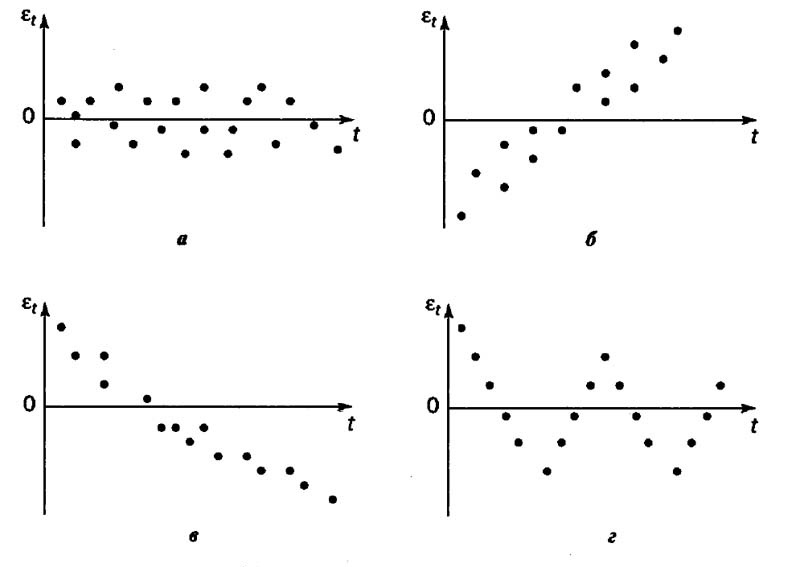
\includegraphics[width=0.24\paperwidth]{ostatki_t.jpg}
На картинке (а) изображен график нормальных остатков по времени. На всех остальных изображены графики остатков с различными видами автокорреляции. \\

\underline{\textsc{\textit{Второй способ}}}: Проведение тестов на выявление автокорреляции. \\
\begin{itemize}
\item \textbf{Тест серий}. \\
\\
Для проведения теста выписываются знаки остатков по очереди, при этом \textit{серия} -- набор остатков одного знака. \\
\textit{Дано:} $T$ -- общее число наблюдений, $N_1$ -- число положительных остатков, $N_2$ -- число отрицательных остатков, $K$ -- число серий.
$$H_0: \text{нет автокорреляции}$$
$$H_a: \text{положительная автокорреляция/отрицательная автокорреляция}$$
Если $K \le K_{min}$ -- автокорреляция положительная; \\
Если $K \ge K_{max}$ -- автокорреляция отрицательная. \\
При этом $K_{min} = \min\{N_1;N_2\}-1$, $K_{max} = \max\{N_1,N_2\}+1$.\\
Если $T>40$, справедливо следующее:
$$K\overset{as}{{\sim}}N(\frac{2N_1N_2}{N_1+N_2}+1;\frac{2N_1N_2(2N_1N_2-N_1-N_2)}{(N_1+N_2)^2(N_1+N_2-1)})$$
\\
\item \textbf{Тест Дарбина - Уотсона}. \\
\\
В этом тесте используется особая статистика, которая так и называется -- статистика Дарбина - Уотсона (DW-статистика). Рассчитывается она следующим образом:
$$DW=\frac{\sum\limits_{t=2}^T(e_t-e_{t-1})^2}{\sum\limits_{t=1}^T e_t^2}\approx2-2\rho,\:|\rho|<1\Rightarrow0< 2-2\rho<4$$
\columnbreak

Тестирование на автокорреляцию с помощью DW-статистики проводится по следующей гипотезе:
$$H_0: \rho=0 \text{, т.е. отсутствие автокорреляции}$$
$$H_a: \rho>0 \; \text{ЛИБО}\;\rho<0$$
Для проведения расчетов используются две вспомогательные переменные $d_u$ и $d_L$, значения которых заданы таблично. При этом: $0<d_L<d_u<2$. \\
\\
\underline{При $H_a: \rho>0$ (положительная автокорреляция):} \\
1)$DW<d_L\Rightarrow$ Присутствует положительная автокорреляция. \\
2)$d_L \le DW \le d_U \Rightarrow$ Определить наличие автокорреляции невозможно. \\
3)$DW>d_U  \Rightarrow$ Положительная автокорреляция отсутствует. \\
\\
\underline{При $H_a: \rho<0$ (отрицательная автокорреляция:} \\
1)$DW>(4-d_L)\Rightarrow$ Присутствует отрицательная автокорреляция. \\
2)$(4-d_U)\leq DW\leq (4-d_L)\Rightarrow$ Определить наличие автокорреляции невозможно.\\
3)$DW<(4-d_U)\Rightarrow$ Отрицательная автокорреляция отсутствует. \\

\item \textbf{Тест Бройша - Годфри}. \\
\\
В отличие от предыдущих тестов, этот тест используется для выявления автокорреляции более 1-го порядка. \\
\\
Пусть $y_t=\beta_1+\beta_2x_t+\varepsilon_t$, при этом $\;$ $\varepsilon_t=\rho_1\varepsilon_{t-1}+\rho_2\varepsilon_{t-2}+\dotsc+\rho_p\varepsilon_{t-p}+u_t$ \\
Гипотеза выглядит следующим образом:
$$H_0: \rho_1=\dotsc=\rho_p=0 \text{ (автокорреляции в остатках нет)}$$
$$H_a: \exists\rho_j\neq0,\:j=1\dotsc T \text{ (автокорреляция есть)}$$
\textit{Шаг 1.} Оценивается начальная модель и рассчитывается ряд остатков. \\
\textit{Шаг 2.} Оценивается дополнительная модель:
$$e_t=\beta_1+\beta_2x_t+r_1e_{t-1}+r_2e_{t-2}+\dotsc+r_pe_{t-p}+u_t$$
\textit{Шаг 3.} Для дополнительной модели рассчитывается $R^2_{e}$, а затем статистика вида:
$$\chi^2 = T\times R^2_{e}\sim\chi^2_p$$
Если значение статистики превышает критическое при выбранном уровне значимости, основная гипотеза об отсутствии автокорреляции отвергается.

\end{itemize}

\subsection*{\textbf{11.3 Что делать, если обнаружилась автокорреляция?}}
\begin{itemize}

\item \textbf{Переход к взвешенным разностям.} \\
Пусть модель выглядит как $y_t = \beta_1 + \beta_2x_t + \varepsilon_t$.\\
\textit{Шаг 1.} Необходимо получить оценку параметра $\rho$. Например, можно оценить его из статистики Дарбина-Уотсона по формуле $\hat{\rho}=1-\frac{d}{2}$. \\
\textit{Шаг 2.} Далее исходное уравнение сдвигается на шаг назад и домножается на $\rho$:
$$\rho y_{t-1}=\rho \beta_1 + \rho \beta_2x_{t-1}+\varepsilon_{t-1}$$
\textit{Шаг 3.} Вычесть из исходного уравнения преобразованное. Получаем: $$y_t-\rho y_{t-1} = \beta_1(1-\rho) +\beta_2(x_t - \rho x_{t-1}) + \varepsilon_t - \rho \varepsilon_{t-1}$$
Теперь автокорреляция отсутствует, но теряется одно наблюдение.\\

\item \textbf{Поправка Прайса - Уинстона.} \\
Заменяем первые наблюдения:\\
$$y^*_1 = y_1\sqrt{1-\rho^2}, \quad x^*_1 = x_1\sqrt{1-\rho^2}$$


\end{itemize}
\section*{12.0 Временные ряды}
\begin{tcolorbox}[colback=red!5!white,colframe=red!75!black]
\textbf{Временной ряд} -- ряд некоторых числовых величин, измеренных в последовательные моменты времени.
$${\{y_t\}}^{+\infty}_{-\infty},\:t=1\dotsc T$$
\end{tcolorbox}
Ключевым отличием временных рядов от пространственных выборок является то, что наблюдения строго упорядочены по времени, невозможно произвольно менять их местами, а также выкидывать из выборки.

\subsection*{\textbf{12.1 Стационарные процессы}}
\begin{tcolorbox}[colback=blue!5!white,colframe=blue!75!black]
\textbf{\underline{Утверждение 12.1}} \textbf{$\{y_t\}$} называется стационарным в узком смысле, если распределение $y_{t1},y_{t2},y_{t3},\dotsc,y_{tk}$ совпадает с распределением $y_{t1+s},y_{t2+s},y_{t3+s},\dotsc,y_{tk+s}$ \: $\forall t_1\dotsc t_{k+s},\:s>0, k>0$
\end{tcolorbox}

\begin{tcolorbox}[colback=blue!5!white,colframe=blue!75!black]
\textbf{\underline{Утверждение 12.2}} \textbf{$\{y_t\}$} называется стационарным в широком смысле, если:
$$\E(y_t)=\mu$$
$$\Var(y_t)=\sigma^2$$
$$\Cov(y_t,y_{t-k})=\Cov(y_{t+s},y_{t-k+s})=\gamma(k)$$
\end{tcolorbox}

Стационарный временной ряд -- это такой ряд, который не меняется со временем с каким-либо трендом, то есть не растет и не снижается. Формально это означает, что математическое ожидание стационарного временного ряда -- постоянно, равно как и его дисперсия, а его значения на равном расстоянии друг от друга связаны одинаково.

\subsection*{\textbf{12.2 Процессы AR, MA, ARMA и ARIMA}}

\begin{tcolorbox}[colback=green!5!white,colframe=green!75!black]
\textbf{\underline{Определение 12.0}} Белый шум $y_t \sim WN(0, \sigma^2)$ -- слабо стационарный процесс, обладающий следующими свойствами:
$$E(y_t)=E(y_s)=0$$
$$\Var(y_t) = Var(y_s) = \sigma^2 $$
$$\Cov(y_t,y_s) = 0$$
\end{tcolorbox}

\begin{tcolorbox}[colback=red!5!white,colframe=red!75!black]
\textbf{\underline{Определение 12.1}} $AR(p)$ -- процесс, зависящий только от своих предыдущих значений и ошибки в текущий момент времени: $$y_t = c + \alpha_1y_{t-1} + \alpha_2y_{t-2}+...+\alpha_py_{t-p} + \varepsilon_t = c + \sum\limits_{i=1}^p \alpha_iy_{t-i} + \varepsilon_t$$
$$t=1,...,T; \quad \varepsilon_t \sim WN(0, \sigma^2)$$
\end{tcolorbox}

\begin{tcolorbox}[colback=red!5!white,colframe=red!75!black]
\textbf{\underline{Определение 12.2}} $MA(q)$ -- процесс, зависящий только от лагов случайной ошибки: $$y_t = c +  \varepsilon_t + \beta_1\varepsilon_{t-1}+...+\beta_q\varepsilon_{t-q}= c + \sum\limits_{i=1}^q \beta_i\varepsilon_{t-i} + \varepsilon_t$$
$$t=1,...,T; \quad \varepsilon_t \sim WN(0, \sigma^2)$$
\end{tcolorbox}

\begin{tcolorbox}[colback=red!5!white,colframe=red!75!black]
\textbf{\underline{Определение 12.3}} $ARMA(p,q)$ -- процесс, зависящий и от своих предыдущих значений, и от текущей и предыдущих ошибок: $$y_t = c +  \sum\limits_{i=1}^p \alpha_iy_{t-i} + \sum\limits_{j=1}^q \beta_j\varepsilon_{t-j} + \varepsilon_t$$
$$t=1,...,T; \quad \varepsilon_t \sim WN(0, \sigma^2)$$
\end{tcolorbox}

\underline{\textit{Как выбрать оптимальное число лагов?}} Можно использовать информационные критерии Акаике (AIC) и Шварца (BIC):
$$AIC(p,q) = \ln\hat{\sigma}^2+2\frac{p+q+1}{T} \longrightarrow \min\limits_{p,q}$$
$$BIC(p,q) = \ln\hat{\sigma}^2 +\frac{p+q+1}{T}\ln T \longrightarrow \min\limits_{p,q}$$
\\
Также можно провести тесты Льюнг - Бокса и Бокса - Пирса.\\ Оба проверяют следующую гипотезу:
$$H_0: \text{процесс - } WN(0,\sigma^2)$$
$$H_a: \text{процесс - } ARMA(p,q) $$
\textbf{1. Q-тест Льюнг - Бокса.} Статистика рассчитывается как:
$$Q_k = T(T+2)\sum\limits_{k=1}^K \frac{1}{T-K}r^2_k \sim \chi^2_{K-p-q-1}$$
\textbf{2. Q-статистика Бокса - Пирса.} Статистика рассчитывается как:
$$Q_k = T\sum\limits_{k=1}^K r^2_k \sim \chi^2_{K-p-q-1}$$
В обоих случаях, если при выбранном уровне значимости величина статистики превышает критическое значение, основная гипотеза отвергается.\\


\begin{tcolorbox}[colback=red!5!white,colframe=red!75!black]
\textbf{\underline{Определение 12.4}} Если для некоторого ряда $y_t$ необходимо взять $d$ разностей, чтобы привести его к стационарному виду, а ряд $\Delta y_t$ описывается моделью $ARMA(p,q)$, то ряд $y_t$ описывается моделью $ARIMA(p,d,q)$.
\end{tcolorbox}

\subsection*{\textbf{12.3 Тест Дики - Фуллера на стационарность ряда}}
Для начала необходимо привести исходный ряд к виду \\
$\Delta y_t=\delta+\gamma t + (\theta-1)y_{t-1} + \varepsilon_t$, где $\delta$ -- константа, а $\gamma t$ отвечает за тренд. Гипотеза формулируется как:
$$H_0: \theta-1=0 \:\text{- ряд нестационарный}$$
$$H_a: \theta-1<0 \:\text{- ряд стационарный}$$
При этом предполагается, что $\varepsilon_i \sim N(0, \sigma^2)$.\\
Тестовая статистика (DF-статистика) рассчитывается по формуле, аналогичной с формулой t-статистики на значимость коэффициента:
$$DF=\frac{\hat{\theta}-1}{\sqrt{\hat\Var(\hat{\theta}-1)}}$$
\\
У статистики Дики-Фуллера своя таблица критических значений и свое распределение, если тестовая статистика находится правее критического значения, то нулевая гипотеза отвергается. При этом критическое значение рассчитывается исходя из спецификации теста: \\
1. Без константы; \\
2. С константой; \\
3. С константой и трендом.

\subsection*{\textbf{12.4 Ложная корреляция и коинтеграция}}
\begin{tcolorbox}[colback=green!5!white,colframe=green!75!black]
\textbf{Ложная корреляция} -- эффект, при котором между двумя переменными наблюдается значимая корреляция, при этом отсутствует качественная причинно-следственная связь. Может возникать из-за того, что обе переменные являются нестационарными, и в них обеих наблюдается стохастический тренд.
\end{tcolorbox}

\begin{tcolorbox}[colback=green!5!white,colframe=green!75!black]
\textbf{Коинтеграция} -- свойство нескольких нестационарных временных рядов, заключающееся в существовании некоторой их стационарной линейной комбинации.
\end{tcolorbox}
Говорят, что нестационарный ряд является интегрированным порядка $d$, если необходимо взять $d$ разностей, чтобы его к стационарному виду. Такие ряды означаются как $I(d)$. \\
\begin{tcolorbox}[colback=blue!5!white,colframe=blue!75!black]
Рассмотрим два нестационарных ряда: $y_t\sim I(d)$ и $x_t\sim I(d)$,где $I(d)$. Если существует такой вектор $(\alpha,\beta):\alpha\neq0,\:\beta\neq0$, что $\alpha y_t+\beta x_t\sim I(d-b), b>0$, то ряды называются \textit{коинтегрированными} порядка b.
\end{tcolorbox}
%\subsubsection*{\textbf{12.4.1 Тест Энгла - Гренджера на коинтеграцию}}
%\textit{Дано}: $y_t\sim I(1)$ и $x_t\sim I(1)$ \\
%Тест проверяет наличие коинтеграции у двух временных рядов. При этом обязательным условием является то, что оба ряда -- интегрированные первого порядка. Строится парная регрессия вида:
%$$y_t=\alpha_1 + \alpha_2 x_t + \varepsilon_t$$
%Остатки этой регрессии проверяются на стационарность тестом, аналогичным тесту Дики - Фуллера, с той лишь разницей, что критические значение Энгла - Гренджера находятся левее (для них также существует отдельная таблица). Если для остатков гипотеза о наличии единичного корня не отвергается, то коинтеграции нет.

\end{multicols}
\end{document}
